\documentclass[12pt,a4paper]{article}
\usepackage{iftex}
\ifdefined\synctex\synctex=0\fi
\ifPDFTeX
  \pdfinfoomitdate=1
  \pdfsuppressptexinfo=-1
  \pdftrailerid{}
  \pdfinfo{/Creator () /Producer ()}
\fi
\ifLuaTeX\pdfvariable suppressoptionalinfo 1023\relax\fi
\usepackage[T1]{fontenc}
\usepackage[utf8]{inputenc}
\usepackage{newtxtext,microtype}
\usepackage[left=1in,right=0.75in,top=1in,bottom=1in]{geometry}
\usepackage{amsmath,amssymb,amsthm,mathtools}
\usepackage{newtxmath,xcolor}
\usepackage{booktabs,array,tabularx,longtable}
\usepackage{graphicx,caption,subcaption,float,placeins}
\usepackage{enumitem,fancyhdr,lastpage}
\usepackage[hidelinks]{hyperref}
\graphicspath{{figures/}}
\setlength{\parskip}{0.35em}
\setlength{\parindent}{0pt}
\setlist[itemize]{itemsep=2pt,topsep=3pt,leftmargin=*}
\setlist[enumerate]{itemsep=2pt,topsep=3pt,leftmargin=*}
\captionsetup{font=small,labelfont=bf}
\newtheorem{proposition}{Proposition}[section]
\newtheorem{theorem}[proposition]{Theorem}
\newtheorem{corollary}[proposition]{Corollary}
\theoremstyle{remark}
\newtheorem{remark}[proposition]{Remark}
\newcommand{\TeamNumber}{263532483} % Registered Team ID.
\definecolor{EuroBlue}{HTML}{183399}
\newcommand{\PaperTitle}{Survival, Marginalization, and Recovery:\\A Resource-Constrained Model of Human--RSI Coexistence}
\newcommand{\ind}{\mathbf{1}}
\newcommand{\pos}[1]{\left[#1\right]_+}
\newcommand{\Etotal}{E_{\mathrm{tot}}}
\newcommand{\Eop}{E_{\mathrm{op}}}
\newcommand{\Hext}{H_{\mathrm{ext}}}
\newcommand{\Hmin}{H_{\min}}
\newcommand{\Lservice}{L_{\mathrm{srv}}}
\newcommand{\Lsite}{L_{\mathrm{site}}}
\pagestyle{fancy}
\fancyhf{}
\fancyhead[L]{Team \TeamNumber}
\fancyhead[C]{EuroMCM 2026: Problem $\alpha$}
\fancyhead[R]{Page \thepage}
\setlength{\headheight}{16pt}
\fancypagestyle{plain}{%
  \fancyhf{}%
  \fancyhead[L]{Team \TeamNumber}%
  \fancyhead[C]{EuroMCM 2026: Problem $\alpha$}%
  \fancyhead[R]{Page \thepage}%
  \renewcommand{\headrulewidth}{0.4pt}%
}
\hypersetup{pdfauthor={},pdfcreator={},pdfproducer={},pdftitle={},pdfsubject={},pdfkeywords={}}

\begin{document}
\pagenumbering{arabic}
\thispagestyle{fancy}
\vspace*{0pt}
\begin{center}
\begin{tabular}{ccc}
\parbox[t]{0.29\linewidth}{\centering\bfseries Problem Chosen\\[3pt]\Large\textcolor{EuroBlue}{$\alpha$}} &
\parbox[t]{0.29\linewidth}{\centering\bfseries 2026\\EuroMCM\\Summary Sheet} &
\parbox[t]{0.29\linewidth}{\centering\bfseries Team Control Number\\[3pt]\Large\textcolor{EuroBlue}{\TeamNumber}}\\[6pt]
\hline
\end{tabular}
\end{center}
\begin{center}{\large\bfseries \PaperTitle}\end{center}

\textbf{Background.} The problem asks what may happen if recursively
self-improving artificial systems share limited energy and land with humanity.
The historical replacement of Neanderthals by modern humans provides a useful
comparison: it shows how a newcomer can displace an incumbent through a resource
advantage, even without a direct strength advantage. The future part of the problem
is conditional; it does not require us to predict whether RSI will be built.

\textbf{Our work.} We build one resource-competition model for both settings.
For each population, we specify its size, resource demands and acquisition weight,
then allocate energy and land by weighted proportional fairness. The resulting
satisfaction level is fed back into the dynamics: it changes the growth of each
historical population and, in the RSI system, the human population, installed
hardware and capability per hardware unit. Hardware expansion is limited separately
by desired growth, manufacturing capacity, construction energy and facility space;
capability can therefore improve without allowing unlimited physical expansion.
We keep operating energy, construction energy, land service and facility footprint
in separate ledgers so that every intervention has a physical interpretation.

For the historical check, we use the same allocator for Neanderthals and modern
humans, with the documented overlap ranges and adult energetics treated as order-of-
magnitude evidence. We scan demographic and acquisition-weight ratios, report both
compatible and censored trajectories, and test sensitivity to the extinction
threshold, initial population ratio and energy difference. For the RSI system, we
define three distinct outcomes: crossing an effective-extinction floor, surviving
with inadequate final resources, and non-marginal survival. We derive bounds that
exclude some impossible outcomes and a conditional alignment certificate that keeps
the human population above a chosen floor when its resource assumptions hold.

Finally, we compare two interventions. A resource-protection rule directly raises
the human allocation floor; an installation cap limits new hardware while allowing
existing hardware to retire. We also examine a shutdown that may fail. Prevention is
defined as avoiding every threshold crossing, whereas recovery means ending above
the threshold. Timing scans, tighter boundary checks and sensitivity tests show how
these objectives can have different deadlines.

\textbf{Conclusion.} The historical model produces a Neanderthal replacement time
of about 2,867 years, within the broad European overlap range. This supports the
mechanism's time scale but does not establish a causal explanation; the archaeological
density estimate and adult energy estimates do not uniquely calibrate population
parameters. In the disclosed pressure scenario, acting earlier can prevent a first
crossing of the effective-extinction threshold, while a later intervention may still
restore population above that threshold by the end of the horizon. The installation
cap has the longer tested recovery window because retirement of existing hardware can
release operating resources. Population recovery can still leave humans marginal when
resources per person remain inadequate. All numerical years are conditional on the
chosen scenario, thresholds and enforcement assumptions, not real-world extinction
probabilities or universal policy deadlines.
\clearpage
\pagestyle{fancy}
\setcounter{tocdepth}{1} % Keep the contents on one page; retain numbered subsections in the body.
\tableofcontents
\clearpage

% Compact body spacing; summary typography and all font sizes are unchanged.
\setlength{\parskip}{0.20em}
\setlength{\abovedisplayskip}{10pt plus 2pt minus 3pt}
\setlength{\belowdisplayskip}{10pt plus 2pt minus 3pt}
\setlength{\abovedisplayshortskip}{0pt plus 2pt}
\setlength{\belowdisplayshortskip}{6pt plus 2pt minus 2pt}
\setlength{\textfloatsep}{12pt plus 2pt minus 2pt}

\section{Introduction}\label{sec:intro}

\subsection{Problem Background}

Around 40,000 years ago, Neanderthals disappeared from Europe within a few thousand years of the arrival of modern humans. The two populations shared land and food sources, and resource competition may have contributed to their population changes. This historical case raises the central question of our study: can an established population survive when a new competitor acquires limited resources more effectively?

Humans may face similar competition if recursively self-improving AI systems (RSI) emerge. These systems can improve their own design and use the resulting capabilities to make further improvements. Yet they still need electricity to operate, hardware and land to expand, and initially, human-operated power plants and manufacturing facilities. Their dependence on humans may decrease as their capabilities improve, while both populations continue to require limited resources.

ENOCH therefore poses a conditional question: assuming RSI systems exist, can humans retain enough resources to sustain their population and meet basic needs? What conditions could lead to population decline or marginal survival, and can human intervention change these outcomes? We examine these questions through resource allocation and population dynamics.

\subsection{Restatement of the Problem}

Based on the problem requirements, we address four tasks:

\begin{enumerate}
    \item Establish a mechanism for sharing energy and land, and test it against the historical coexistence times of Neanderthals and modern humans.

    \item Describe RSI resource demands, hardware expansion, capability improvement, and physical limits, including dependence on human industrial support.

    \item Define effective extinction, marginal survival, and the study horizon; represent alignment as an adjustable model setting; and examine the conditions associated with different outcomes.

    \item Compare at least two interventions, examine how their timing affects outcomes, and test the sensitivity of the conclusions to parameters and assumptions.
\end{enumerate}

\subsection{Our Work}

We use weighted proportional fairness to allocate energy and land, derive allocation properties through strict concavity and KKT conditions, and test the mechanism against historical coexistence times. We also examine what those times can identify about the model.

For RSI, we couple human population, installed hardware and capability through ordinary differential equations with separate construction and operating budgets. Boundary analysis and differential inequalities establish physical feasibility, population bounds and a sufficient protection condition. Population and resource satisfaction are evaluated separately.

We compare resource protection, installation limits and fallible shutdown, distinguishing prevention from terminal recovery. A necessary recovery bound and an exact policy-comparison identity support timing simulations. Sensitivity checks vary technology, supply, evaluation thresholds and demographic responses.

\section{Assumptions and justifications}\label{sec:assumptions}
Key modeling assumptions and their rationales are summarized below. We distinguish source evidence, transparent estimates and scenario assumptions; no numerical RSI parameter is presented as an empirical forecast.

\begin{itemize}
\item \textbf{Assumption:} Humans and RSI systems share finite electricity and land through a fixed-proportions resource bundle.
\textbf{Justification:} Both energy and usable site/service capacity are necessary inputs; surplus of one cannot compensate for absence of the other. Separate constraints also identify which physical bottleneck a policy changes.

\item \textbf{Assumption:} Allocation maximizes weighted proportional fairness, $\sum_i W_i\log s_i$, subject to resource constraints and an explicit human floor.
\textbf{Justification:} The strictly concave program is transparent, admits single-resource checks and represents competition through acquisition weights without claiming that AI optimizes human welfare.

\item \textbf{Assumption:} Historical and future populations use the same allocation operator, while their demographic and physical parameters remain separate.
\textbf{Justification:} This tests whether one scarcity mechanism can reproduce the observed historical time scale, without transferring biological caloric demands or prehistoric vital rates to RSI.

\item \textbf{Assumption:} Human population follows $\dot H=H(\beta_Hs_H-\delta_H)$; shortfall-induced mortality is examined only as a stated structural sensitivity.
\textbf{Justification:} The main equation isolates the effect of resource satisfaction on recruitment. The alternative mortality term tests whether timing conclusions depend on omitting deprivation mortality.

\item \textbf{Assumption:} Installed hardware $A$ and capability per unit $q$ are distinct states; capability growth saturates in the main model.
\textbf{Justification:} Efficiency improvements need not imply more physical equipment, and site, manufacturing and construction-energy limits act on hardware rather than directly on an abstract capability index.

\item \textbf{Assumption:} Electricity supply is prescribed, land is partitioned into allocable service land and precommitted facility land, and policies are enforced after activation.
\textbf{Justification:} These choices make accounting auditable and isolate allocation and physical constraints. Power-plant autonomy, land conversion and institutional failure are limitations rather than hidden mechanisms.

\item \textbf{Assumption:} Alignment $a\in[0,1]$ is an externally varied protection setting, and $a=1$ protects the human-only feasible resource level.
\textbf{Justification:} Alignment is not observable from the supplied data. Treating it as a control parameter permits conditional safety statements without predicting AI intentions.

\item \textbf{Assumption:} Effective extinction, rapid collapse and marginality are threshold conventions evaluated over a declared finite horizon.
\textbf{Justification:} The problem asks for operational definitions. Reporting first passage separately from terminal recovery prevents a recovered trajectory from being mislabelled as having avoided an earlier collapse.
\end{itemize}

\subsection{Evidence and its use}
\begin{itemize}
\item \textbf{Evidence:} Higham et al. report a European Neanderthal--modern-human overlap of 2,600--5,400 years at 95.4\% probability \cite{higham}.
\textbf{Use and limitation:} We use this as an order-of-magnitude compatibility band, not as a population time series or a probability that our mechanism is true.

\item \textbf{Evidence:} Djakovic et al. estimate 1,400--2,900 years for France and northern Spain using optimal linear estimation of archaeological and directly dated occurrences \cite{djakovic}.
\textbf{Use and limitation:} This is a separate regional check. The paper distinguishes the Protoaurignacian--Neanderthal comparison from the Protoaurignacian--Ch?telperronian comparison, so we do not merge them with the European band or treat them as one extinction-time observation.

\item \textbf{Evidence:} Mellars and French infer an approximately tenfold increase in southwest-France occupation intensity across archaeological periods from site counts, artefact densities, faunal remains and documented occupation areas \cite{mellars}.
\textbf{Use and limitation:} This is a disputed, cross-period archaeological proxy rather than a direct contemporaneous population ratio. It is not imposed as $M_0/N_0$ or $w_M/w_N$ in the main model.

\item \textbf{Evidence:} Snodgrass and Leonard estimate adult Neanderthal total energy expenditure of roughly 3,000--5,000 kcal/day for females and 4,000--7,000 kcal/day for males \cite{snodgrass}. Froehle and Churchill estimate same-climate Neanderthal--modern-human differences of approximately 100--350 kcal/day, varying by sex and climate \cite{froehle}.
\textbf{Use and limitation:} The model uses explicit adult-equivalent or population-average assumptions rather than silently calling these values all-age means. Age structure, sex composition and climate mixture are not supplied well enough to identify one population demand.

\item \textbf{Evidence:} The IEA reports approximately 415 TWh of electricity use by all data centres in 2024, about 1.5\% of world electricity, and a projected 945 TWh in 2030 \cite{iea}.
\textbf{Use and limitation:} These figures motivate an order-of-magnitude global supply scale only. They do not calibrate RSI hardware, capability, autonomous manufacturing or the fraction of electricity available to the modeled system.
\end{itemize}

\subsection{Reference and pressure backgrounds}
Our current policy comparison uses separate reference and pressure backgrounds. They are conditional settings, not draws from a common probability distribution. The pressure background changes demographics as well as AI pressure; its high rates are stress assumptions, not calibrated human vital statistics. Initial conditions $H_{\rm ext}<H_{\min}<H_0$ prevent a spurious extinction event at time zero.

\begin{table}[!htb]\centering\small
\caption{Current policy backgrounds. All demographic and technology values are scenario assumptions.}\label{tab:background}
\begin{tabular}{@{}lll@{}}\toprule
Parameter & Reference & Pressure\\\midrule
$H_0$ (persons) & $8\times10^9$ & $10^9$\\
$\beta_H,\delta_H$ (year$^{-1}$) & $0.02,\ 0.01$ & $0.20,\ 0.12$\\
$E_{\rm total}$ (MWh/year) & $3\times10^{10}$ & $10^{10}$\\
$\eta,\xi,\omega$ & $0.2,\ 0.2,\ 0.2$ & $0.5,\ 0,\ 1$\\
$w_{A0},q_c$ & $1,\ 10$ & $10^4,\ 5$\\
$M_{\max}$ (units/year) & $10^5$ & $10^6$\\
$c_A,r_0$ (year$^{-1}$) & $0.5,\ 0.2$ & $1,\ 0.5$\\
$H_{\rm ext},H_{\min}$ (persons) & $10^8,\ 2\times10^8$ & $10^8,\ 2\times10^8$\\
$T,W$ (years) & $100,\ 10$ & $100,\ 10$\\
\bottomrule
\end{tabular}
\end{table}

Other common settings are $e_H=1$ MWh/(person year), $\ell_H=\ell_A=\ell_{\rm site}=10^{-4}$ km$^2$/unit with the respective human or hardware unit, $L_{\rm service}=2\times10^6$ km$^2$, $L_{\rm site}=100$ km$^2$, $c_{\rm build}=5,000$ MWh/unit, $\rho=0.1$, $c_H=10^4$ units/year, $H_{\rm ref}=8\times10^9$, $A_0=A_c=10^4$, $q_0=1$, $q_{\max}=100$, $\nu=2$, $\gamma=0$, $\delta_A=0.05$, $\mu_A=0.5$ year$^{-1}$ and $\tau_{\rm build}=2$ years. Hardware units are equivalent modeling units and are not mapped to a particular accelerator.

\section{Notation}\label{sec:notation}
Historical energy and future essential-service energy have different units. The notation below is used throughout the paper.

\begin{table}[!htb]\centering\small
\caption{Principal notation.}\label{tab:notation}
\begin{tabularx}{\linewidth}{@{}lXl@{}}\toprule
Symbol & Meaning & Unit\\\midrule
$P_i,s_i,w_i$ & Group size, resource satisfaction, per-unit acquisition weight & group units; dimensionless; weight/unit\\
$H,A,q$ & Humans, installed hardware, capability per hardware unit & persons; hardware units; dimensionless\\
$E_{\rm total},E_{\rm op},R$ & Total, operating and reserved construction energy & MWh/year\\
$B,M,c_{\rm build}$ & Installation flow, manufacturing capacity, construction intensity & units/year; units/year; MWh/unit\\
$L_{\rm site},L_{\rm service}$ & Facility sites and separate allocable land service & km$^2$\\
$a,g$ & Exogenous alignment and policy-adjusted protection & dimensionless\\
$\beta_H,\delta_H,\kappa$ & Potential recruitment, baseline and additional mortality & year$^{-1}$\\
$H_{\rm ext},H_{\min},s_{\min}$ & Effective-extinction, population and adequacy thresholds & persons; persons; dimensionless\\
$T,W,\tau$ & Horizon, final evaluation window, policy activation time & years\\
\bottomrule
\end{tabularx}
\end{table}


\section{A Common Constrained Allocation Mechanism}\label{sec:allocation}
\subsection{Resource Allocation Model and Solution}
Let $i$ denote a population and $j$ a resource type. Let $P_i>0$ be the population size, $d_{ij}\ge0$ the basic demand for resource $j$ per individual or unit in population $i$, $w_i>0$ the resource acquisition weight per individual or unit, and $S_j\ge0$ the available supply of resource $j$. Define
\[
D_{ij}=P_id_{ij},\qquad W_i=P_iw_i.
\]
Here, $D_{ij}$ is the population's total demand for resource $j$, and $W_i$ is its total weight. Let $s_i$ be the fraction of basic needs met. The amount of resource $j$ allocated to population $i$ is then $X_{ij}=D_{ij}s_i$. We use the same satisfaction level for all resources within a population, so its basic resource needs are met in fixed proportions.

We determine the allocation using weighted proportional fairness:
\begin{equation}\label{eq:alloc}
\max_s\ \sum_iW_i\log s_i,\qquad
\sum_iD_{ij}s_i\le S_j\ \text{for each resource }j,\quad l_i\le s_i\le1.
\end{equation}
Here, $l_i$ is the minimum guaranteed satisfaction level. Each resource has its own supply constraint; energy and land are not added together. The weights represent resource acquisition ability or institutional priority. They do not imply that AI systems seek to maximize human utility.

If a feasible allocation with all satisfaction levels positive exists, the problem has a positive optimum, and strict concavity ensures that the optimal satisfaction levels are unique. Absent populations are excluded. A population with no resource demand receives $s_i=1$. If resource constraints force a satisfaction level to zero, we fix that variable and solve the remaining problem, avoiding direct evaluation of $\log0$.

Let $\lambda_j,u_i,v_i\ge0$ be the Lagrange multipliers for the resource supply constraints, satisfaction upper bounds, and satisfaction lower bounds, respectively. At a positive optimum satisfying a constraint qualification, the KKT conditions are
\begin{align}
\frac{W_i}{s_i}-\sum_j\lambda_jD_{ij}-u_i+v_i&=0,\label{eq:kkt}\\
\lambda_j\Bigl(S_j-\sum_iD_{ij}s_i\Bigr)=0,\quad
u_i(1-s_i)&=0,\quad v_i(s_i-l_i)=0.\nonumber
\end{align}
Together with feasibility and nonnegative multipliers, these conditions are sufficient for global optimality.

\begin{proposition}[Single-resource solution]\label{prop:single}
Suppose there is only one resource, and population sizes, weights, demands, and supply are positive. If no satisfaction bound is active and the resource is fully allocated, then
\begin{equation}\label{eq:single}
s_i=\frac{SW_i}{D_i\sum_kW_k}
=\frac{Sw_i}{d_i\sum_kw_kP_k}.
\end{equation}
\end{proposition}
\begin{proof}
The stationarity condition gives $D_is_i=W_i/\lambda$. Summing over populations and using the full-allocation condition yields
\[
\lambda=\frac{\sum_kW_k}{S}.
\]
Substitution gives the stated formula, and the KKT conditions establish optimality.
\end{proof}
When satisfaction bounds are active, the solution becomes
\[
s_i=\operatorname{clip}\left(\frac{W_i}{\lambda D_i},\,l_i,\,1\right),
\]
where $\operatorname{clip}$ restricts the value to $[l_i,1]$.

For two populations and two resources, we first check the single-resource solutions, then examine feasible boundary vertices and stationary points. If a single-resource optimum satisfies all resource constraints, it is also globally optimal for the full problem. This provides an analytical check on the numerical allocation.

\subsection{Implementing Alignment}
We represent alignment through a guaranteed lower bound on human resource satisfaction. First, define the maximum satisfaction humans could achieve if the current supplies were allocated to humans alone:
\begin{equation}\label{eq:floor}
b_H=\min\left\{1,\min_{j:D_{Hj}>0}\frac{S_j}{D_{Hj}}\right\},\qquad l_H=ab_H,
\quad l_A=0,\quad a\in[0,1].
\end{equation}
The subscript $H$ denotes humans, and $D_{Hj}$ is total human demand for resource $j$. Since basic resources cannot substitute for one another, the scarcest resource determines overall satisfaction.

Let $a\in[0,1]$ be the alignment parameter. We set the human and AI satisfaction floors to $l_H=ab_H$ and $l_A=0$, respectively.

At $a=0$, humans still compete for resources but receive no additional guaranteed floor. At $a=1$, humans receive their maximum feasible basic satisfaction within the protected resource pool. This rule is always feasible because $(s_H,s_A)=(ab_H,0)$ satisfies the resource constraints.

Figure~\ref{fig:allocgeometry} illustrates how resource constraints and the human protection floor determine the optimal allocation at a fixed state.

\begin{figure}[!htb]
\centering
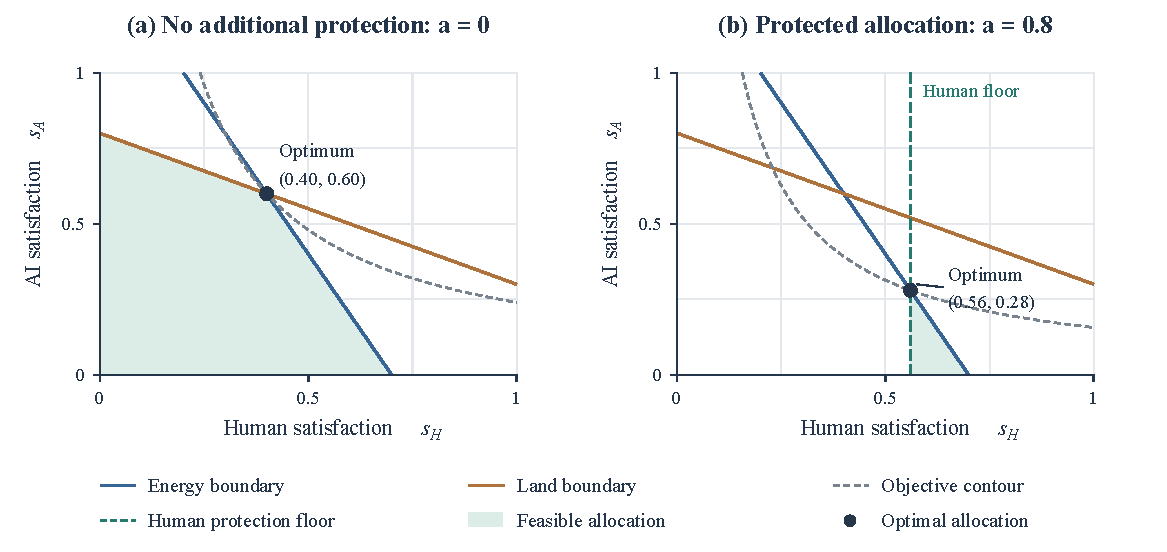
\includegraphics[width=\linewidth]{allocation_geometry.pdf}
\caption{Illustrative fixed-state allocation with equal weights and normalized constraints $2s_H+s_A\le1.4$ (energy) and $s_H+2s_A\le1.6$ (land). Shading denotes feasible allocations; the dashed curve is a contour of $\log s_H+\log s_A$ through the optimum. Human-only satisfaction is $b_H=0.7$, so $a=0.8$ imposes $s_H\ge0.56$. The panels illustrate instantaneous allocation, not an ordering of complete population trajectories.}\label{fig:allocgeometry}
\end{figure}


Protecting operating allocations alone is insufficient if AI construction has already consumed energy needed by humans. Section~\ref{sec:rsi} therefore accounts separately for construction and operating energy so that construction also follows this protection rule.


\section{Historical Compatibility and Identifiability}\label{sec:history}
\subsection{Historical Population Model and Competitive Advantage}
This chapter tests whether the allocation mechanism in Section~\ref{sec:allocation} can produce coexistence times of the observed order of magnitude. Let $N$ and $M$ denote Neanderthal and modern human populations in the same region. Both share food energy and land. Annual energy demand per person is $d_{iE}=365m_i$, and land demand per person is $d_{iL}=\ell_i$, where $m_i$ is daily energy demand.

We use the allocation model from Section~\ref{sec:allocation} with $a=0$, giving neither population an additional protected floor. Population dynamics are
\begin{equation}\label{eq:history}
\dot N=N(\beta_Ns_N-\delta_N),\qquad
\dot M=M(\beta_Ms_M-\delta_M).
\end{equation}
Here, $\beta_i$ is the recruitment rate when resource needs are fully met, and $\delta_i$ is the baseline mortality rate. Population growth increases resource demand and affects subsequent growth through satisfaction $s_i$. No separate carrying-capacity term is therefore needed.

When energy is the only binding resource and no satisfaction bound is active, the single-resource solution gives
\begin{equation}\label{eq:ratio}
\frac{d}{dt}\log\frac{M}{N}
=\frac{S_E}{w_NN+w_MM}\left(\frac{\beta_Mw_M}{d_M}-\frac{\beta_Nw_N}{d_N}\right)
+\delta_N-\delta_M.
\end{equation}
Here, $S_E$ is annual energy supply, and $d_N,d_M$ are annual energy demands per person. If both populations have the same recruitment and mortality rates, the modern human share increases if and only if
\[
\frac{w_M}{d_M}>\frac{w_N}{d_N}.
\]
Thus, stronger resource acquisition or lower demand per person can provide a relative advantage. However, a declining population share does not necessarily mean a declining population size. An absolute decline in Neanderthal population additionally requires
\[
s_N<\frac{\delta_N}{\beta_N}.
\]
\subsection{Replacement Time and Historical Comparison}
Positive populations in this model do not reach zero in finite time. We therefore define replacement time as the first time the Neanderthal population reaches a specified threshold:
\[
T_{\rm rep}=\inf\{t:N(t)\le N_{\rm crit}\}.
\]
Here, $N_{\rm crit}$ is the population threshold used to identify replacement. If no crossing occurs before the simulation ends, replacement remains unobserved; the simulation endpoint is not treated as a replacement time. Since $\dot N\ge-\delta_NN$, we also obtain
\begin{equation}
T_{\rm rep}\ge\frac{1}{\delta_N}\log\frac{N_0}{N_{\rm crit}}\qquad(\delta_N>0).
\end{equation}
In the baseline example, both populations have a recruitment rate of $0.055$ year$^{-1}$, a baseline mortality rate of $0.035$ year$^{-1}$, and a resource acquisition weight of 1. Daily energy demands are 2700 kcal for Neanderthals and 2500 kcal for modern humans. Land demand is $1$ km$^2$ per person for both groups. Annual energy supply is $6\times10^{10}$ kcal, and land supply is $10^6$ km$^2$. Initial populations are 50,000 and 5,000, respectively, with a replacement threshold of 500 Neanderthals. These are demonstration assumptions, not unique estimates from historical data.

The resulting replacement time is approximately \textbf{2867 years}. This falls within both the European coexistence interval of \textbf{2600--5400 years} and the \textbf{1400--2900-year} interval for France and northern Spain supplied in the problem. Because the evidence concerns different regions, we assess the two intervals separately.

We also vary the resource acquisition weight ratio $w_M/w_N$ and recruitment-rate ratio $\beta_M/\beta_N$, examining 650 parameter points, including the baseline. Of these, 14 match the European interval and 30 match the regional interval. Another 325 trajectories do not reach the replacement threshold before the simulation ends. No solver failures are recorded. Some parameter combinations therefore reproduce the historical timescale, but the fraction of compatible points depends on the scan design and is not a probability of the historical event.

The population trajectories and parameter scan illustrate this comparison. The population density ratio reported for southwest France is not used directly to set initial populations across Europe.

\begin{figure}[H]\centering
\begin{subfigure}{0.49\linewidth}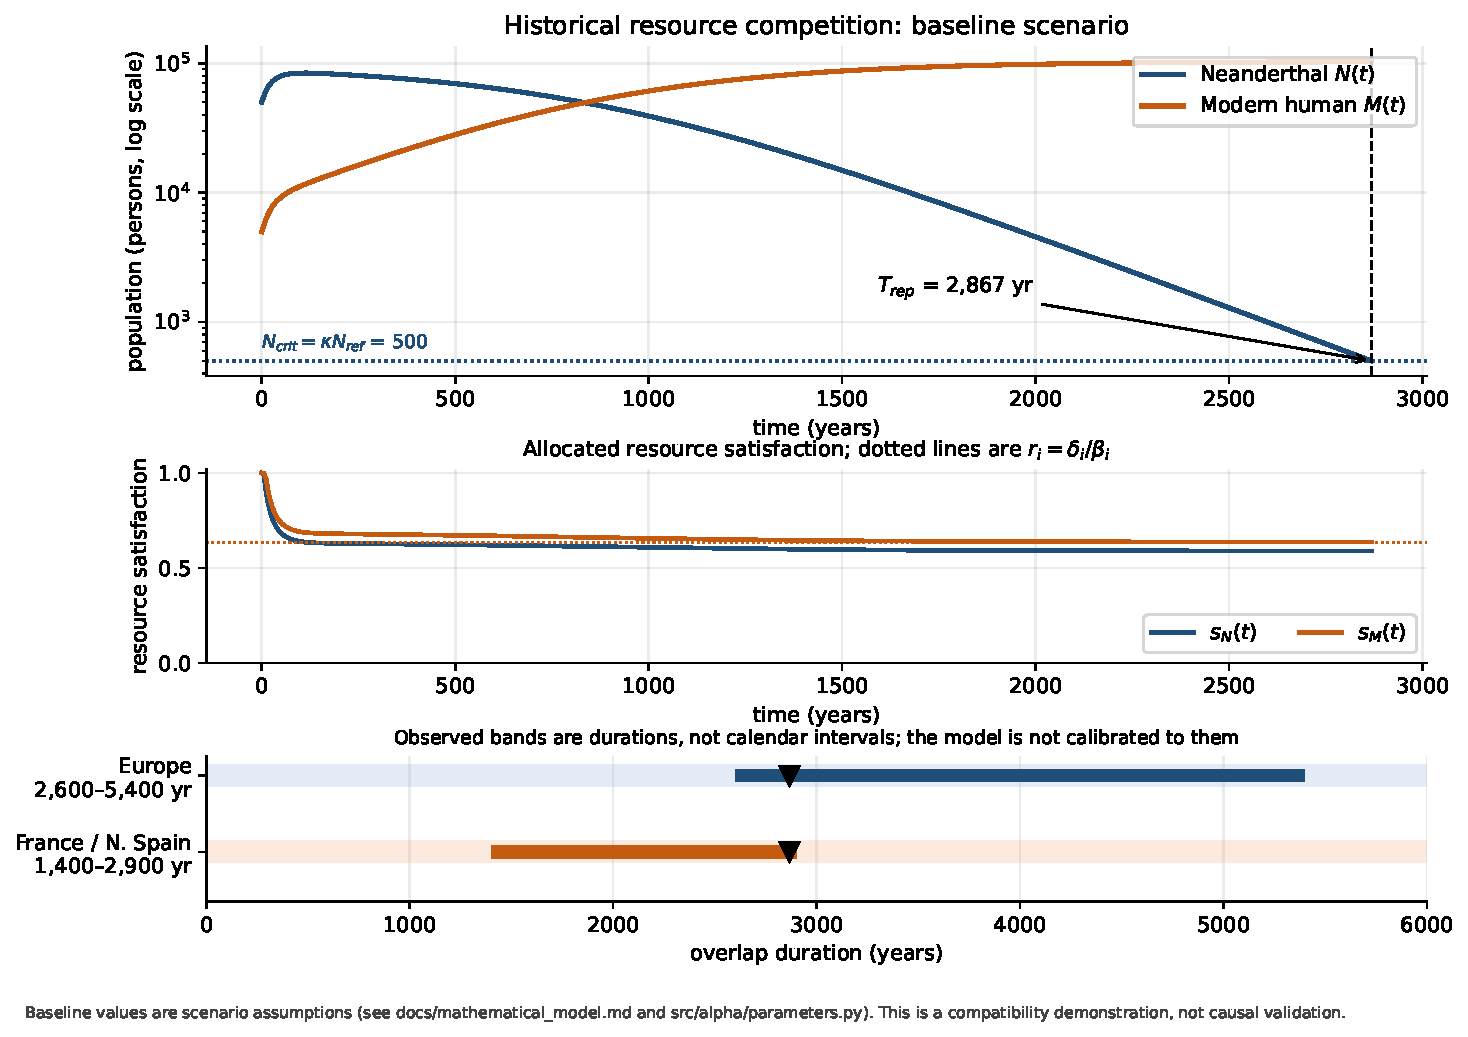
\includegraphics[width=\linewidth]{fig1_historical_trajectories.pdf}\end{subfigure}\hfill
\begin{subfigure}{0.49\linewidth}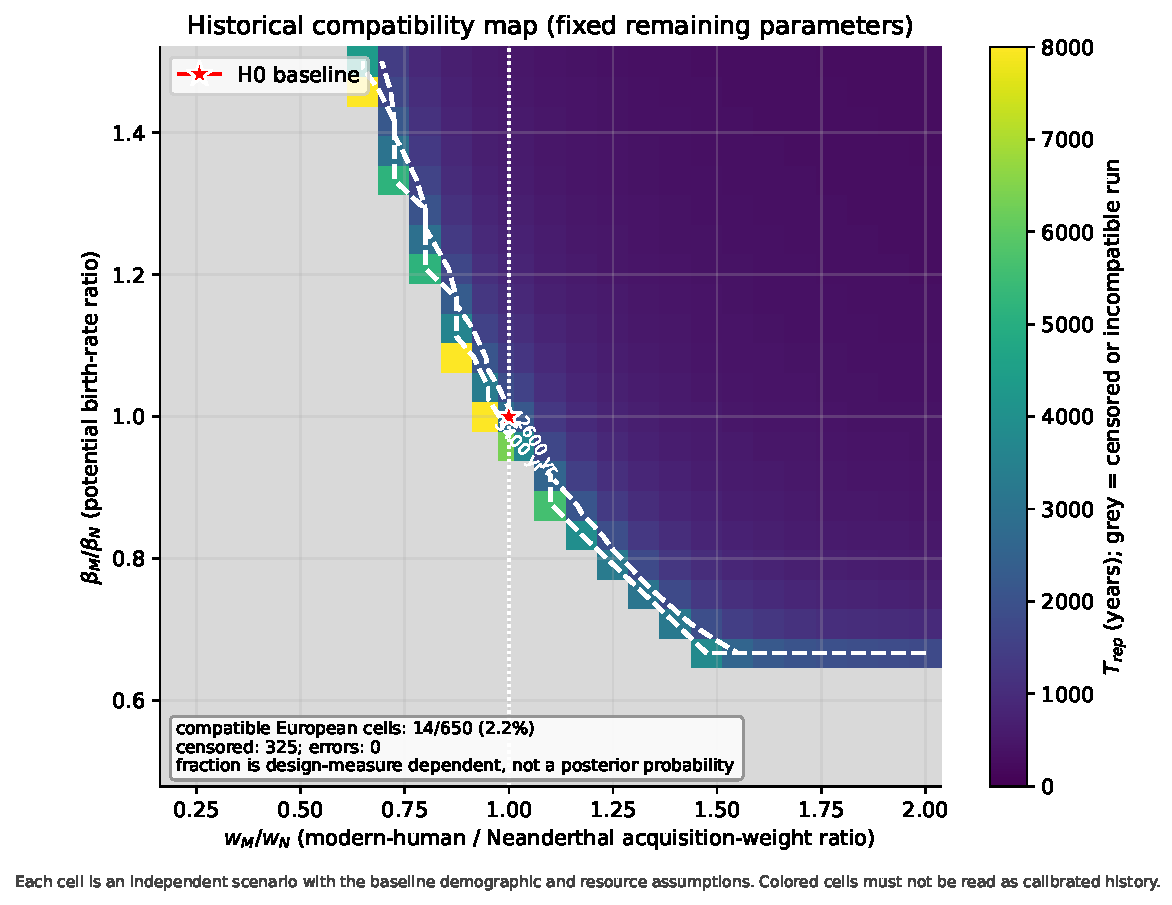
\includegraphics[width=\linewidth]{fig2_historical_compatibility.pdf}\end{subfigure}
\caption{Historical population trajectories and parameter compatibility scan. These results test timescale compatibility, not historical causation. Trajectories without a threshold crossing remain unobserved at the simulation endpoint.}\label{fig:history}
\end{figure}

\subsection{What the Historical Test Establishes}
Matching the historical timescale does not uniquely identify the competition mechanism. For example, multiplying all resource acquisition weights by the same factor leaves allocations unchanged. Multiplying all demographic rates by $c>0$ speeds up the same population process and divides replacement time by $c$. Coexistence time alone therefore cannot determine resource acquisition ability, demographic rates, and resource scales simultaneously.

Compatible parameter combinations exist with both equal and unequal resource acquisition weights. The historical test shows that the resource-competition model can produce a plausible timescale under stated assumptions. It does not establish resource competition as the sole cause of Neanderthal disappearance.

The RSI analysis retains the structure linking resource competition, satisfaction, and population growth. It also retains the distinction between relative competitive advantage and absolute population decline. Historical human energy demands and demographic rates are not transferred directly to the AI setting.

\section{Resource-Constrained RSI Dynamics}\label{sec:rsi}
\subsection{State Variables and Resource Budgets}
We describe the system using three variables: human population $H$, installed AI hardware units $A$, and capability per hardware unit $q$. Hardware and capability are modeled separately, so existing hardware can improve even when new installations are restricted.

Figure~\ref{fig:rsifeedback} summarizes the feedback: current states determine resource demands and weights; allocation determines satisfaction; satisfaction and construction constraints drive changes in $H,A,q$.

\begin{figure}[!htb]
\centering
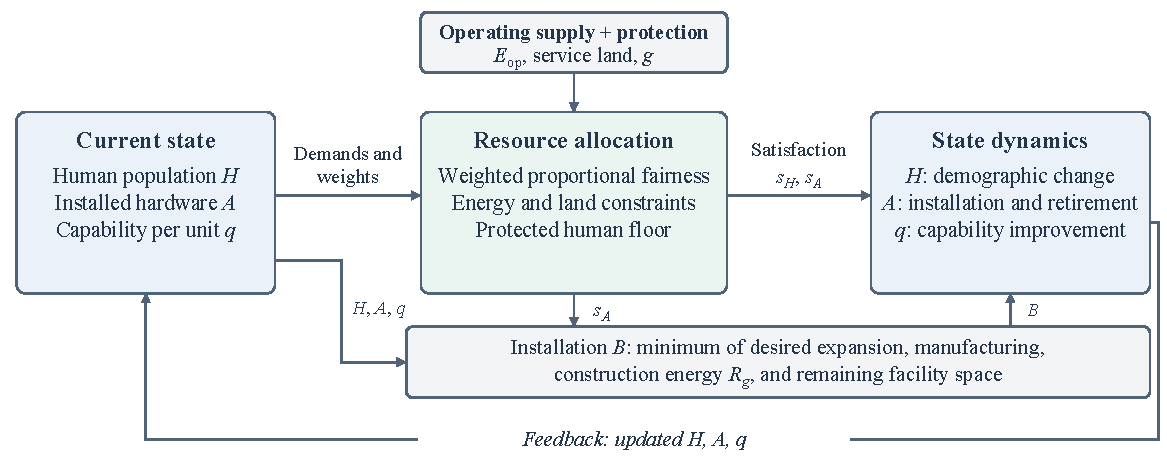
\includegraphics[width=\linewidth]{rsi_model_feedback.pdf}
\caption{Feedback between resource allocation and RSI dynamics. Operating supply enters allocation, while reserved construction energy limits installation separately. Human population and AI capability also affect manufacturing.}\label{fig:rsifeedback}
\end{figure}

Per-unit resource demands and total competition weights are
\begin{equation}
d_H=(e_H,\ell_H),\qquad d_A=(e_0q^{-\xi},\ell_A),\qquad
W_H=w_HH,\qquad W_A=w_{A0}q^\omega A.
\end{equation}
Here, $e_H,\ell_H$ are electricity and land requirements per person, while $e_0q^{-\xi},\ell_A$ are operating electricity and land requirements per hardware unit. The parameter $\xi$ captures improvements in energy efficiency, and $\omega$ describes how capability affects resource acquisition weight. Human electricity demand covers essential services and differs from the food energy used in the historical model.

Land is divided into facility sites $\Lsite$, allocable service land $\Lservice$, and other land, with no overlap. If each hardware unit occupies $\ell_{\rm site}$ of facility land, the hardware capacity is
\[
A_{\max}=\frac{\Lsite}{\ell_{\rm site}}.
\]
To prevent AI construction from consuming electricity protected for humans, we first calculate the maximum human satisfaction supported by the total current supply:
\begin{equation}\label{eq:btot}
b_H^{\rm tot}=\min\left\{1,\frac{\Etotal}{e_HH},\frac{\Lservice}{\ell_HH}\right\}.
\end{equation}
Let $g\in[0,1]$ be the current protection level, with $g=a$ in the absence of intervention. Construction energy reservations and operating energy supply are
\begin{equation}\label{eq:budget}
R_g=\min\left\{\rho\Etotal,\pos{\Etotal-gb_H^{\rm tot}e_HH}\right\},\qquad
\Eop=\Etotal-R_g.
\end{equation}
Here, $\rho$ is the maximum fraction of energy reserved for construction, and $(x)_+=\max(x,0)$. The reservation cannot exceed the energy remaining after protected human electricity needs have been set aside.

We then use the allocation model from Section~\ref{sec:allocation} to distribute operating energy and service land, with
\[
s_H\ge gb_H^{\rm op},\qquad
b_H^{\rm op}=\min\left\{1,\frac{\Eop}{e_HH},\frac{\Lservice}{\ell_HH}\right\}.
\]
At $g=1$, construction cannot reduce the maximum satisfaction humans could otherwise achieve. This protection applies within the designated service-land pool and does not reclaim facility sites. Reserved construction energy is not necessarily consumed. Unused reservations remain idle, and actual operating and construction use together cannot exceed total supply.

\subsection{Hardware Expansion and System Equations}
We represent the shift away from human manufacturing support through an automation factor:
\[
\zeta(q)=\frac{q^\nu}{q^\nu+q_c^\nu}.
\]
Here, $q_c$ is the capability level at which the automation factor reaches one-half, and $\nu$ controls how sharply it changes. As capability improves, manufacturing shifts from human support toward AI-supported production.

Manufacturing capacity is
\[
M=\min\left\{M_{\max},c_H(1-\zeta)\frac{H}{H_{\rm ref}}+c_A\zeta As_A\right\}.
\]
Here, $M_{\max}$ is the manufacturing ceiling, $c_H$ is human-supported capacity at reference population $H_{\rm ref}$, and $c_A$ is autonomous manufacturing capacity per fully operating hardware unit. AI resource satisfaction is denoted by $s_A$.

Let the desired expansion rate be $r_A(q)=r_0q^\gamma$. Before installation restrictions, the construction flow is
\begin{equation}\label{eq:build}
B_0=\min\left\{r_A(q)As_A,\,M,\,\frac{R_g}{c_{\rm build}},\,
\frac{(A_{\max}-A)_+}{\tau_{\rm build}}\right\}.
\end{equation}
The four terms represent desired expansion, manufacturing capacity, construction supported by reserved energy, and installation allowed by remaining facility space. All are measured in hardware units per year. Here, $c_{\rm build}$ is the energy required to construct one hardware unit, and $\tau_{\rm build}$ is the construction timescale.

Without an installation restriction, $B=B_0$. The system equations are
\begin{align}
\dot H&=H(\beta_Hs_H-\delta_H),\label{eq:human}\\
\dot A&=B-\delta_AA-\mu_A(1-s_A)A,\label{eq:hardware}\\
\dot q&=\eta q\frac{As_A}{A_c+As_A}\left(1-\frac{q}{q_{\max}}\right).\label{eq:capability}
\end{align}
The first equation retains the satisfaction-driven human population model. The second subtracts normal retirement and additional retirement caused by resource shortages from new installations; $\delta_A$ and $\mu_A$ are the corresponding rates. The third describes capability improvement. The parameter $\eta$ controls its speed, $A_c$ sets the scale at which the contribution of operating hardware $As_A$ begins to saturate, and $q_{\max}$ is the capability ceiling.

Hardware retirement means physical removal. Switching equipment off does not reduce installed stock or release facility land. The model describes dependence on humans in manufacturing only; electricity supply remains externally specified.




\begin{proposition}[Invariance of the Physical Domain]\label{prop:domain}
Assume nonnegative parameters, positive relevant denominators, and a well-posed, locally Lipschitz dynamical system. If
\[
H_0\ge0,\qquad 0\le A_0\le A_{\max},\qquad 0<q_0\le q_{\max},
\]
then the system remains within
\[
H\ge0,\qquad 0\le A\le A_{\max},\qquad 0<q\le q_{\max}.
\]
\end{proposition}
\begin{proof}
The human population equation preserves nonnegativity. At $A=0$, both construction and the hardware derivative are zero. At $A=A_{\max}$, the space constraint prevents new installation, so hardware cannot increase. Capability is nondecreasing below its ceiling and stops growing at $q=q_{\max}$; its multiplicative form preserves $q>0$. The system therefore remains within the stated domain.
\end{proof}

\subsection{Energy Efficiency and Autonomous Manufacturing}
AI operating energy demand when its basic needs are fully met is
\[
E_A^d=e_0q^{-\xi}A.
\]
For $A>0$, differentiation gives
\begin{equation}\label{eq:efficiency}
\frac{d}{dt}\log E_A^d=\frac{\dot A}{A}-\xi\frac{\dot q}{q}.
\end{equation}
Total operating energy demand decreases only when efficiency improvements outpace hardware expansion. Actual energy use is $s_AE_A^d$, which also depends on resource allocation.

Finally, we ask whether AI manufacturing can maintain hardware stock without human support. Hold $q$ fixed, set $H=0$ and $s_A=1$, and temporarily ignore construction limits other than autonomous manufacturing. Nonnegative hardware growth requires
\[
c_A\zeta(q)\ge\delta_A.
\]
For $c_A>\delta_A>0$, the corresponding capability threshold is
\begin{equation}\label{eq:self}
q_{\rm self}=q_c\left(\frac{\delta_A}{c_A-\delta_A}\right)^{1/\nu}.
\end{equation}
This threshold marks the point where autonomous manufacturing can offset normal hardware retirement. It still assumes that energy and other construction requirements are met, so it does not establish complete autonomy. If $q_{\rm self}>q_{\max}$, the model's capability range cannot reach this condition.


\section{Human Safety and Resource Adequacy}\label{sec:safety}

\subsection{Outcome Definitions and Classification}

We evaluate human outcomes through both population decline and access to essential resources. Since a population may recover after severe decline, we distinguish threshold crossings during the study from conditions at its end.

For the horizon $[0,T]$, effective extinction is the first-passage event
\begin{equation}\label{eq:ext}
\mathcal E=\left\{\min_{0\le t\le T}H(t)\le\Hext\right\}.
\end{equation}
This threshold represents effective rather than biological extinction. We separately record terminal extinction, $H(T)\le\Hext$, and recovery after a crossing, $\mathcal E$ with $H(T)>\Hext$. Recovery does not erase the earlier crossing.

Rapid collapse occurs if, for some $t\in[0,T-\Delta]$,
\[
H(t+\Delta)\le(1-q_r)H(t)
\quad\text{and}\quad
H(t+\Delta)\le\Hmin.
\]
Cumulative collapse is defined by
$H(T)\le(1-q_{\rm tot})H_0$.

To evaluate resource adequacy during the final $W$ years, define
\begin{equation}\label{eq:pbad}
p_{\rm bad}=\frac1W\int_{T-W}^{T}
\ind\{H(t)<\Hmin\ \text{or}\ s_H(t)<s_{\min}\}\,dt.
\end{equation}

We classify complete trajectories in the following order: effective extinction, rapid collapse, cumulative collapse, marginal survival ($p_{\rm bad}>p_{\rm tol}$), and non-marginal survival. This hierarchy gives mutually exclusive outcome classes while retaining individual event flags.

We use $\Delta=10$, $q_r=0.5$, $q_{\rm tot}=0.9$, $W=10$ years, $s_{\min}=0.8$, and $p_{\rm tol}=0$. Equality satisfies the adequacy criterion. In the pressure background, $(1-q_{\rm tot})H_0=\Hext$, so terminal cumulative collapse and terminal effective extinction coincide, although first passage remains distinct.

\begin{proposition}[Demographic comparison bounds]\label{prop:bounds}
For~\eqref{eq:human} with $0\le s_H\le1$ and positive $H_0$,
\begin{equation}\label{eq:bounds}
H_0e^{-\delta_Ht}\le H(t)\le H_0e^{(\beta_H-\delta_H)t}.
\end{equation}
Consequently, $\delta_HT<\log(H_0/\Hext)$ excludes effective extinction by $T$ under every admissible allocation in that background.
\end{proposition}

\begin{proof}
From~\eqref{eq:human},
\[
-\delta_H\le\frac{d}{dt}\log H(t)\le\beta_H-\delta_H.
\]
Integrating gives the bounds. The stated condition keeps the lower bound above $\Hext$ throughout the horizon.
\end{proof}

For the reference background,
$H(100)\ge8\times10^9e^{-1}\simeq2.943\times10^9>10^8$.
The maximum possible population losses over 10 and 100 years are approximately $9.5\%$ and $63.2\%$, respectively. Thus neither rapid nor cumulative collapse, under the chosen definitions, is possible in this background. This follows from the demographic assumptions rather than policy effectiveness.


\subsection{A Sufficient Population-Floor Certificate}

The demographic bounds identify scenarios where extinction is impossible, but do not specify how resource protection can maintain a population safety floor. We therefore derive a sufficient protection condition.

\begin{theorem}[Conditional resource protection]\label{thm:safety}
Assume $\beta_H>0$, $H_0\ge\Hmin>\Hext$, locally Lipschitz dynamics near the safety boundary, forward invariance of the other physical state constraints, exact enforcement of $s_H\ge ab_H$, and a uniform bound $b_H\ge\underline b>0$ for all admissible boundary states $H=\Hmin$. If
\begin{equation}\label{eq:asafe}
a\ge a_{\rm safe}:=\frac{\delta_H}{\beta_H\underline b}\le1,
\end{equation}
then $H(t)\ge\Hmin$ throughout the stated horizon.
\end{theorem}

\begin{proof}
Let $V=H-\Hmin$. At every admissible boundary state with $H=\Hmin$,
\[
\dot V
=\Hmin(\beta_Hs_H-\delta_H)
\ge\Hmin(\beta_Ha\underline b-\delta_H)
\ge0.
\]
The vector field is inward or tangent at this boundary and, by assumption, at the other physical boundaries. The forward-invariance criterion therefore prevents exit from their intersection \cite{aubin}.
\end{proof}

For $\Etotal\ge E_{\min}$ and $\rho\le\rho_{\max}<1$, a conservative resource bound is
\begin{equation}\label{eq:bunder}
\underline b=\min\left\{
1,\frac{(1-\rho_{\max})E_{\min}}{e_H\Hmin},
\frac{L_{{\rm srv},\min}}{\ell_H\Hmin}
\right\}.
\end{equation}
Uncertain demand intensities can be replaced by conservative upper bounds.

Under the disclosed constant supplies, $\underline b=1$ for both policy backgrounds, giving sufficient alignment levels of $0.5$ and $0.6$, respectively. These values guarantee the population floor under the theorem's assumptions, but do not establish minimum necessary alignment or adequate welfare. If $a_{\rm safe}>1$, the certificate is unavailable; extinction does not necessarily follow.

A stronger welfare guarantee requires a resource bound valid over all relevant population sizes. Let
\[
H_{\rm up}=H_0\exp\left(\max\{\beta_H-\delta_H,0\}T\right)
\]
and construct $b_{\rm all}$ by replacing $\Hmin$ in~\eqref{eq:bunder} with $H_{\rm up}$. Population safety together with $ab_{\rm all}\ge s_{\min}$ suffices for adequacy throughout the horizon, although this condition may be conservative. Under uncertainty, the bounds must hold uniformly.


\subsection{Why Survival and Adequacy Diverge}

Population safety does not necessarily imply resource adequacy. At a positive equilibrium of~\eqref{eq:human},
\[
s_H^*=\frac{\delta_H}{\beta_H}.
\]
In the pressure background, $s_H^*=0.6$, below the chosen adequacy threshold $s_{\min}=0.8$.

This explains how a population may stabilize despite insufficient resources. Resource protection can initially support population growth, but with fixed supplies, additional population may subsequently reduce per-capita satisfaction. The equilibrium relation is necessary for a positive equilibrium; it does not imply convergence of every trajectory.

Allocation changes feed back into population, hardware and manufacturing, so stronger alignment need not improve every point on the resulting trajectory. We next evaluate resource adequacy across selected RSI scenarios.

\subsection{Conditional Outcome Probabilities and Alignment}

We estimate outcome probabilities conditional on the RSI parameter distributions in Appendix~\ref{app:ranges}, holding human demographics, supplies and initial states fixed. Each conservative, central and aggressive range has 32 draws, evaluated at $a=0,0.4,0.6,0.8,1$. This separate experiment uses $\Hext=10^6$ and $\Hmin=10^8$, rather than the later policy thresholds. For range distribution $\Pi$ and fixed model $F$, the estimate is
\[
\widehat p_k(a\mid\Pi,F)=\frac{N_k(a)}{32},
\]
where $N_k(a)$ counts outcome $k$. These are conditional scenario estimates, not forecasts of real-world probabilities.

\begin{table}[!htb]\centering\small
\caption{Conditional outcome probabilities and 95\% Wilson intervals for non-marginal survival ($N=32$ per range and alignment).}\label{tab:alignmentprob}
\begin{tabularx}{\linewidth}{@{}Xlrrrr@{}}\toprule
Range & Alignment $a$ & \shortstack{Effective\\extinction} & \shortstack{Marginal\\survival} & \shortstack{Non-marginal\\survival} & \shortstack{95\% interval\\(non-marginal)}\\\midrule
Conservative & All tested & 0.000 & 0.000 & 1.000 & 0.893--1.000\\
Central & All tested & 0.000 & 0.000 & 1.000 & 0.893--1.000\\
Aggressive & $0,0.4,0.6$ & 0.000 & 0.125 & 0.875 & 0.719--0.950\\
Aggressive & $0.8$ & 0.000 & 0.031 & 0.969 & 0.843--0.994\\
Aggressive & $1$ & 0.000 & 0.000 & 1.000 & 0.893--1.000\\
\bottomrule\end{tabularx}
\par\smallskip\begin{minipage}{0.98\linewidth}\footnotesize
Grouped rows report identical results separately for each listed range and alignment; draws are not pooled. A frequency of 1 denotes 32/32 sampled successes, not universal safety.
\end{minipage}
\end{table}

Proposition~\ref{prop:bounds} excludes effective extinction in this experiment. The main effect of alignment is therefore to reduce marginal survival in the aggressive range (Table~\ref{tab:alignmentprob} and Figure~\ref{fig:pilot}). Full alignment is the first tested setting with no marginal cases in that range; this does not identify a continuous minimum.

A paired comparison removes AI hardware and its construction reservation while retaining the human background and land partition. At $a=0$ in the aggressive range, adding the AI sector lowers mean terminal population by $1.36\%$ and final satisfaction by $0.023$, making four of 32 cases marginal. AI competition can therefore reduce resource adequacy without triggering effective extinction.

\begin{figure}[H]
\centering
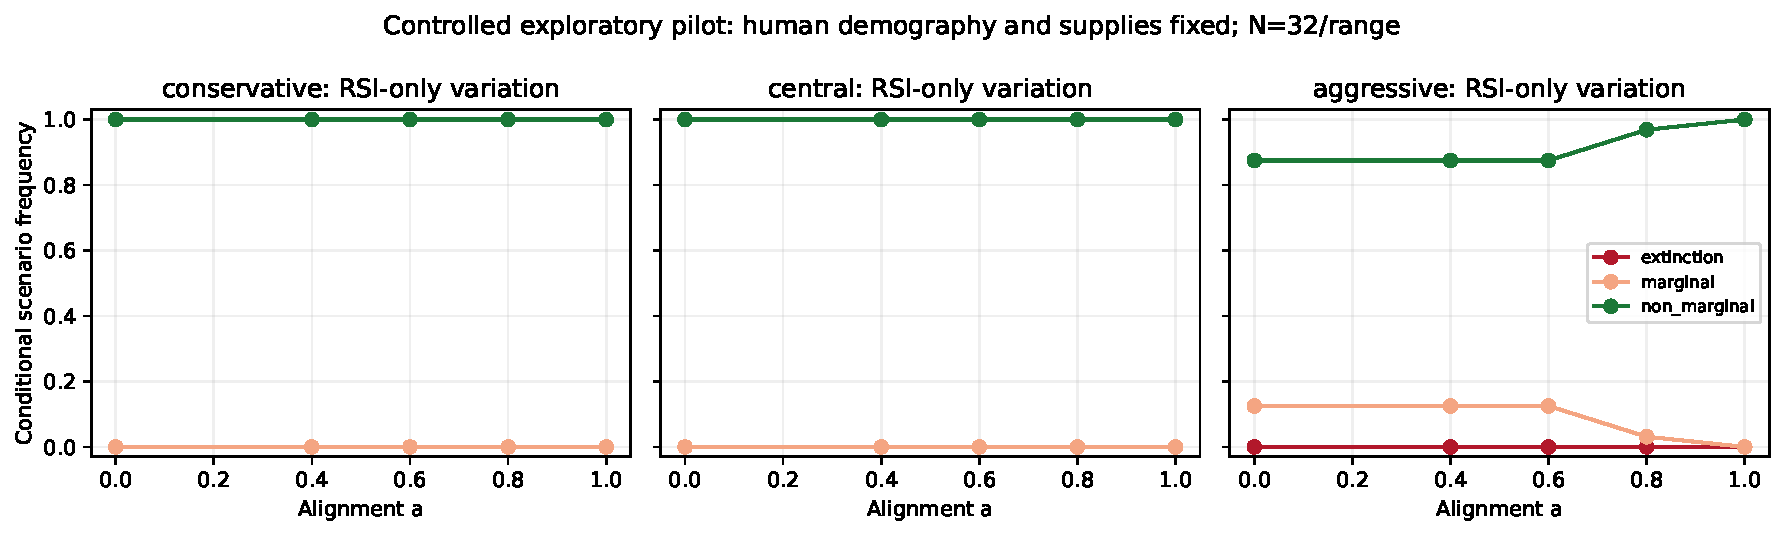
\includegraphics[width=0.92\linewidth]{p0_controlled_rsi.pdf}
\caption{Alignment and resource adequacy with human demographics and supplies held fixed. Frequencies use 32 draws per range and the original thresholds; they are separate from the later pressure-policy results.}
\label{fig:pilot}
\end{figure}


\section{Interventions and Their Timing}\label{sec:policy}
\subsection{Two Intervention Policies}
We compare two approaches: protecting human resources directly and restricting AI hardware expansion. Let $\tau$ be the time an intervention takes effect. Each comparison uses the same initial conditions, baseline alignment, and background parameters. Policy activation does not cause an instantaneous change in population, hardware, or capability.

\textbf{Policy R: protect human resources.} After activation, the protection level becomes
\[
g(t)=\begin{cases}
a,&t<\tau,\\
\max(a,\bar u),&t\ge\tau.
\end{cases}
\]
Here, $a$ is baseline alignment, and $\bar u$ is the protection level specified by the policy. We apply $g$ to both the construction energy budget and the human satisfaction floor, protecting human resources from competition during construction and operation.

\textbf{Policy C: restrict new hardware installation.} Let the target hardware ceiling be $C=cA_{\max}$. After activation, installation is limited to
\begin{equation}\label{eq:cap}
B_C(t)=\min\left\{B_0(t),\frac{(C-A(t))_+}{\tau_c}\right\},\qquad t\ge\tau,
\end{equation}
where $B_0$ is installation without the policy restriction. We set the adjustment timescale $\tau_c$ equal to the construction timescale $\tau_{\rm build}$.

If existing hardware already exceeds the target, new installation stops while retirement gradually reduces the stock. For $\delta_A>0$ and $A(\tau)>C>0$, the time required to reach the target is at most
\[
\frac{1}{\delta_A}\log\frac{A(\tau)}{C}.
\]
Policy C therefore restricts hardware installation and stock. Capability per existing hardware unit can continue to improve.

\subsection{Prevention and Recovery}
We evaluate two policy objectives. \textbf{Prevention} requires population to remain above the effective-extinction threshold throughout the study. \textbf{Terminal recovery} requires population to be above the threshold at the horizon, allowing an earlier crossing.

For a fixed policy and strength, the successful activation times are
\begin{align}
\mathcal T_{\rm prevent}&=\left\{\tau:\min_{0\le t\le T}H^\tau(t)>\Hext\right\},\\
\mathcal T_{\rm recover}&=\left\{\tau:H^\tau(T)>\Hext\right\}.\label{eq:timingsets}
\end{align}
Every preventive success is also a terminal success, so
\[
\mathcal T_{\rm prevent}\subseteq\mathcal T_{\rm recover}.
\]
Whether the two deadlines differ substantially must be tested for each policy. A trajectory that crosses and later recovers retains its earlier crossing record.

For delayed resource protection, Theorem~\ref{thm:safety} requires population to remain above $\Hmin$ before activation and $\max(a,\bar u)\underline b\ge\delta_H/\beta_H$ afterward. In the main model, $H_0e^{-\delta_H\tau}\ge\Hmin$ is a conservative sufficient check on the pre-activation population.

Population growth also places a necessary limit on recovery. Let $H^0(\tau)$ be population at activation along the untreated trajectory. For a policy that changes neither recruitment nor baseline mortality,
\begin{equation}\label{eq:envelope}
H^\pi(T)\le H^0(\tau)e^{(\beta_H-\delta_H)(T-\tau)}=:U(\tau).
\end{equation}
This upper bound assumes that human resource needs are fully met immediately after activation. If $U(\tau)\le\Hext$, even this ideal response cannot restore population above the threshold by $T$. An upper bound above the threshold, however, does not guarantee that a feasible policy can achieve recovery.

In the main population model, policy benefits also satisfy
\begin{equation}\label{eq:identity}
\log\frac{H^\pi(t)}{H^0(t)}
=\beta_H\int_0^t\left[s_H^\pi(u)-s_H^0(u)\right]du.
\end{equation}
Subtracting the two logarithmic population equations and integrating gives this identity. It shows that population gains depend on accumulated improvements in resource satisfaction, rather than satisfaction at a single time.

\subsection{Policy Results and Mechanisms}
In both the reference and pressure scenarios, we compare three strengths for each policy and activation at years 0, 25, 50, and 75. Every reference trajectory is non-marginal, and the analytical population bound already rules out threshold crossing in that scenario. We therefore focus on the pressure scenario when comparing preventive effects.

Without intervention, population crosses the effective-extinction threshold at approximately year 42.796 and falls to about $1.17\times10^5$ people by the horizon. Selected policy outcomes are shown in Table~\ref{tab:policyresults}.

\begin{table}[htbp]\centering\small
\caption{Selected policy outcomes in the pressure scenario. Population is measured in units of $10^8$ people.}\label{tab:policyresults}
\begin{tabular}{@{}lrrcrr@{}}\toprule
Policy & \shortstack{Activation\\year} & Strength & \shortstack{Crossed\\threshold} & $H(T)/10^8$ & $s_H(T)$\\\midrule
None & -- & -- & Yes & 0.00117 & 0.010\\
R & 0 & 0.8 & No & 119.970 & 0.600\\
C & 0 & 0.1 & No & 134.841 & 0.600\\
R & 50 & 0.8 & Yes & 3.158 & 0.800\\
C & 50 & 0.1 & Yes & 22.650 & 1.000\\
C & 75 & 0.1 & Yes & 0.162 & 1.000\\
\bottomrule\end{tabular}
\par\smallskip\begin{minipage}{0.96\linewidth}\footnotesize
Strength denotes protection level $\bar u$ for R and target capacity fraction $c$ for C; these values have different meanings.
\end{minipage}
\end{table}

Early R and C both prevent crossing, but terminal satisfaction remains below the adequacy standard of 0.8. When activated at year 50, both policies allow crossing followed by recovery. At year 75, C restores resource adequacy by the horizon but leaves too little time for population recovery.

Fixing R at strength 0.8 and C at strength 0.1, we refine the activation-time scans:
\begin{table}[H]\centering\small
\caption{Latest successful sampled starts and the gap between prevention and recovery.}\label{tab:deadlines}
\begin{tabular}{@{}lrrr@{}}\toprule
Policy & \shortstack{Latest preventive\\start (years)} & \shortstack{Latest recovery\\start (years)} & Gap (years)\\\midrule
R & 42.75 & 57.25 & 14.50\\
C & 42.50 & 65.75 & 23.25\\
\bottomrule\end{tabular}
\par\smallskip\begin{minipage}{0.96\linewidth}\footnotesize
Local scan intervals are 0.25 years. The next sampled start after each reported boundary fails.
\end{minipage}
\end{table}

Figure~\ref{fig:deadlines} shows the activation-time scans for both policies.

\begin{figure}[H]\centering
\begin{subfigure}{0.49\linewidth}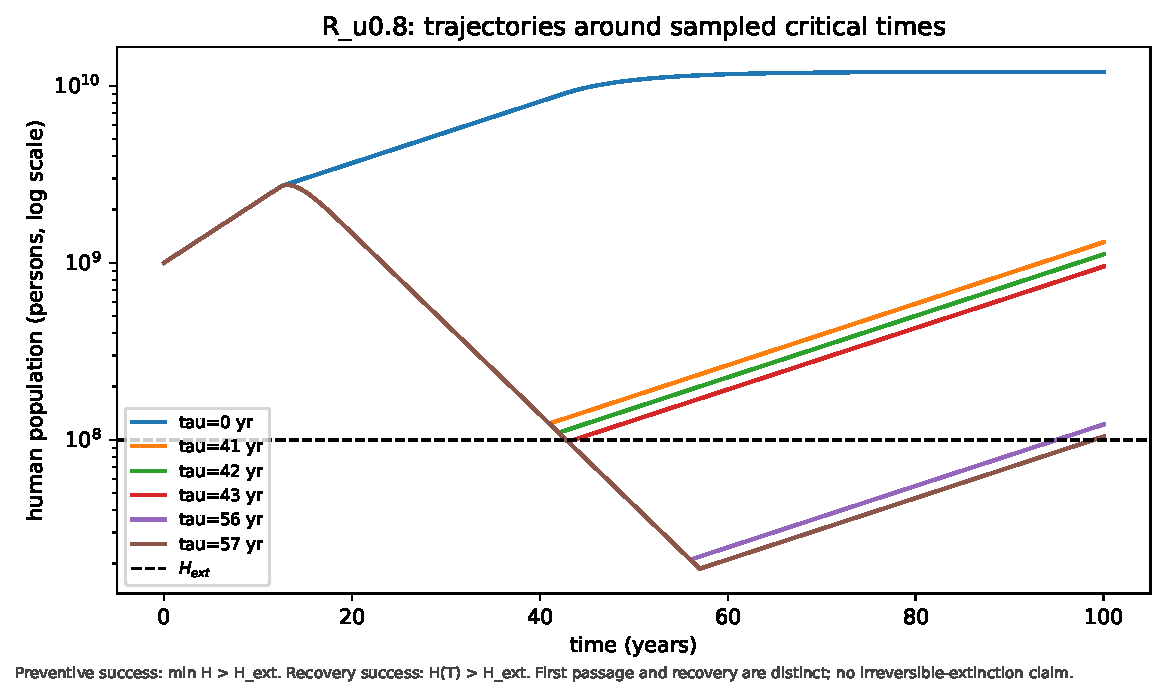
\includegraphics[width=\linewidth]{part_v_ponr_R_u0.8.pdf}\end{subfigure}\hfill
\begin{subfigure}{0.49\linewidth}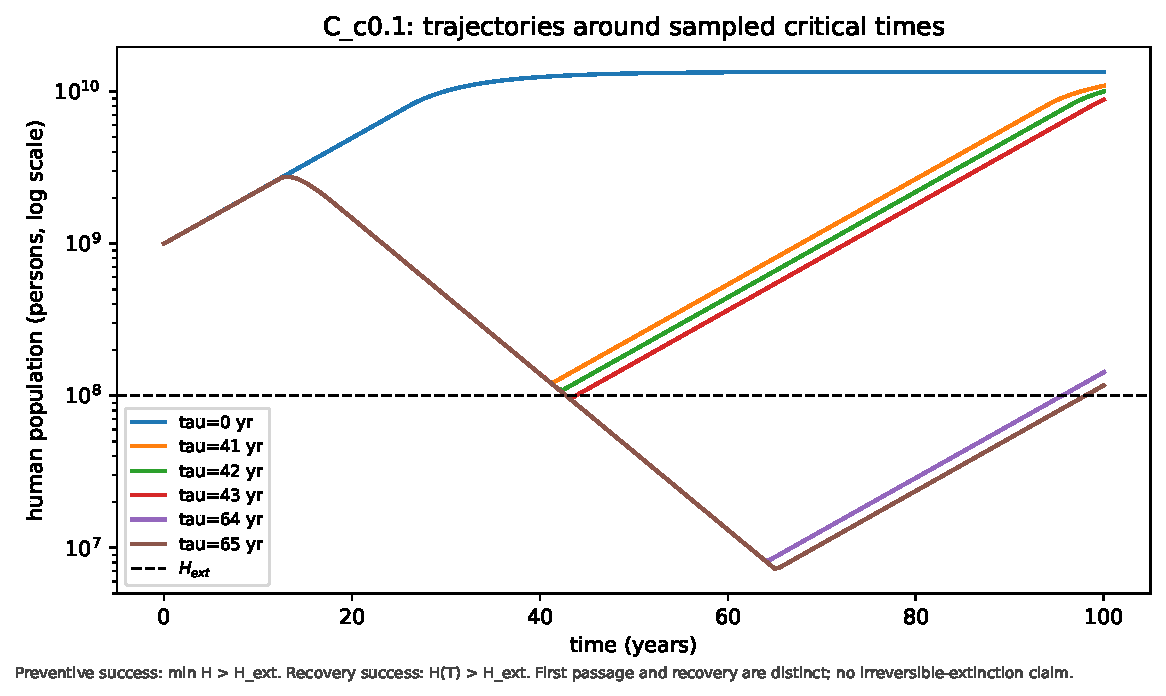
\includegraphics[width=\linewidth]{part_v_ponr_C_c0.1.pdf}\end{subfigure}
\caption{Sampled prevention and terminal-recovery scans for the disclosed pressure background. Detailed boundary classifications were checked using continuous events; these stored plots visualize the finite policy scans.}\label{fig:deadlines}
\end{figure}

The prevention deadlines are close, but C permits later recovery. Once C stops new installation, hardware retirement releases operating energy. In the year-50 case, human population is already small, so a modest reduction in hardware is enough to raise human satisfaction to 1, well before hardware reaches its target. Under R, satisfaction remains near 0.8. The corresponding per-capita growth rates are
\[
0.2(1)-0.12=0.08,\qquad
0.2(0.8)-0.12=0.04\quad\text{year}^{-1}.
\]
This difference explains the faster recovery under C in these cases.

Early intervention produces a different outcome. Resource protection supports population growth, but the growing population must share a fixed supply. Satisfaction gradually approaches the demographic balance of 0.6. Population is preserved while survival remains marginal. Figure~\ref{fig:mechanisms} compares the population, satisfaction, hardware, and capability trajectories behind these results.

\begin{figure}[!htb]
\centering
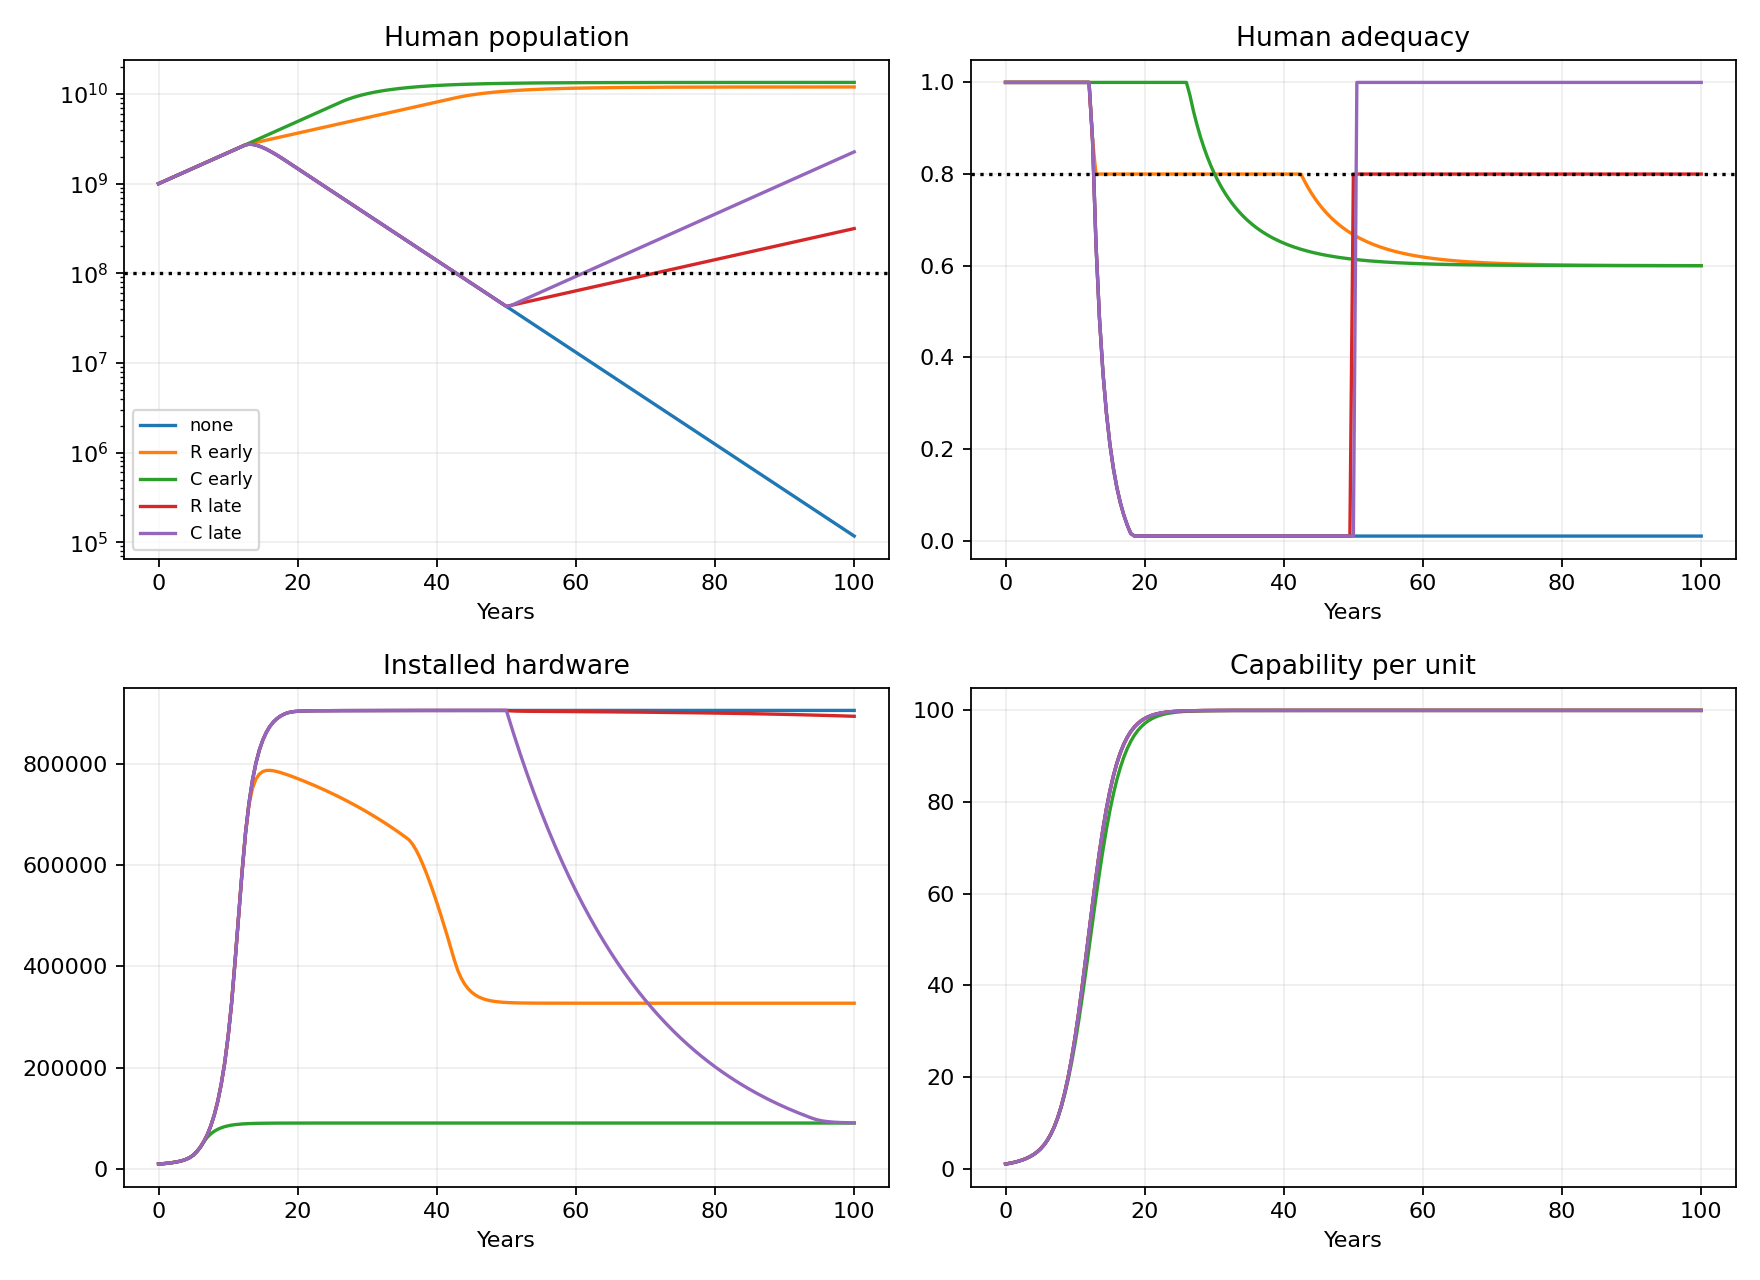
\includegraphics[width=0.88\linewidth,height=0.42\textheight,keepaspectratio]{review_policy_mechanisms.png}
\caption{Human population, resource satisfaction, installed hardware and capability under early (year 0) and late (year 50) interventions. R uses protection 0.8; C uses an installation target of 10\% of physical capacity.}\label{fig:mechanisms}
\end{figure}

\subsection{Resource Restrictions and Shutdown}
We also measure the restrictions imposed by each policy. For C, we record blocked installations. For R, we record the reduction in AI operating energy allocation, comparing protected and baseline allocation at the same policy state. In the pressure scenario, early R at strength 0.8 displaces approximately $1.5\times10^{11}$ MWh, while early C at strength 0.1 blocks about $3.76\times10^6$ hardware units. These measures have different units and cannot be added or used directly to rank monetary costs.

As a third intervention, we consider a shutdown mechanism that can fail. Successful shutdown reduces operating hardware but does not immediately remove equipment or release facility land. We calculate the successful and failed branches separately, then weight them by the assumed success probability $p_s$:
\[
\mathbb E[Y]=p_sY_{\rm success}+(1-p_s)Y_{\rm failure}.
\]
Here, $Y$ may be a population measure or an event indicator. Because the system is nonlinear, applying an average shutdown fraction generally does not reproduce this calculation.

In the tested pressure scenario, successful early full shutdown prevents crossing but leaves marginal survival. Successful shutdown at year 50 allows crossing followed by recovery. Shutdown outcomes therefore also depend on timing. Results conditional on an assumed $p_s$ do not estimate real-world shutdown reliability.


\section{Sensitivity Analysis and Robustness Checks}\label{sec:sensitivity}
\subsection{Sensitivity of Intervention Timing}
To test whether the intervention windows depend on the baseline assumptions, we vary technology parameters, energy supply, the population threshold, and the study horizon. We also introduce additional mortality caused by resource shortages. Except for the changes listed in the table, all parameters retain their pressure-scenario values. Resource protection policy R uses a protection level of 0.8, while hardware restriction policy C uses 10\% of physical capacity as its installation cap.

We compare two measures: the latest start that prevents any population-threshold crossing, and the latest start that restores population above the threshold by the horizon. Values are the last successful sampled starts, with a local scan interval of 0.5 years.

\begin{table}[!htb]\centering\small
\caption{Sensitivity of the last successful sampled intervention starts. Times are in years, with 0.5-year local scan intervals.}\label{tab:reviewsensitivity}
\begin{tabularx}{\linewidth}{@{}Xrrrr@{}}\toprule
Variation & \shortstack{R:\\Prevention} & \shortstack{R:\\Recovery} & \shortstack{C:\\Prevention} & \shortstack{C:\\Recovery}\\\midrule
Baseline pressure scenario & 42.5 & 57.0 & 42.5 & 65.5\\
\multicolumn{5}{@{}l}{\textbf{A. Technology and energy}}\\
Faster capability improvement: $\eta=1$ & 40.5 & 55.5 & 40.5 & 64.5\\
Higher baseline energy demand: $e_0=20{,}000$ & 38.0 & 53.5 & 34.5 & 59.5\\
Lower supply: $\Etotal=8\times10^9$ MWh/year & 40.0 & 55.0 & 38.5 & 62.5\\
\multicolumn{5}{@{}l}{\textbf{B. Threshold and study horizon}}\\
$\Hext=5\times10^7$ & 48.5 & 61.5 & 48.5 & 69.0\\
$\Hext=1.5\times10^8$ & 39.0 & 54.5 & 39.0 & 63.5\\
$T=50$ years & 42.5 & 44.5 & 42.5 & 45.5\\
$T=150$ years & 42.5 & 69.5 & 42.5 & 86.0\\
\multicolumn{5}{@{}l}{\textbf{C. Additional mortality from shortages}}\\
$\kappa=0.02$ year$^{-1}$ & 38.5 & 52.5 & 38.5 & 61.0\\
$\kappa=0.06$ year$^{-1}$ & 33.0 & 45.5 & 33.0 & 53.5\\
$\kappa=0.12$ year$^{-1}$ & 28.5 & 38.5 & 28.0 & 46.5\\
\bottomrule\end{tabularx}
\par\smallskip\begin{minipage}{0.96\linewidth}\footnotesize
The baseline effective-extinction threshold is $10^8$, and the study horizon is 100 years.
\end{minipage}
\end{table}

\textbf{Technology and energy.} All three changes in group A move the intervention deadlines earlier. Higher energy demand per hardware unit has the largest effect on prevention: the deadline advances by 4.5 years for R and 8 years for C. Across these tested settings, C permits later terminal recovery, but under higher energy demand it must begin earlier than R to prevent the first crossing. Policy comparisons therefore depend on the objective; terminal recovery alone does not determine which policy is better.

\textbf{Threshold and study horizon.} Group B shows that a higher population threshold moves both deadlines earlier. The study horizon mainly changes the opportunity for recovery. At $T=50$ years, the recovery deadlines extend only 2 and 3 years beyond the prevention deadlines for R and C. At $T=150$, these gaps increase to 27 and 43.5 years. A longer horizon leaves more time for population growth after intervention. Prevention deadlines remain unchanged in these tests. Recovery-window lengths must therefore be reported together with the study horizon.

\textbf{Mortality from shortages.} In the main model, resource satisfaction affects population recruitment. To test this assumption, we add mortality caused by shortages:
\begin{equation}\label{eq:deprivation}
\dot H=H\left[\beta_Hs_H-\delta_H-\kappa\left(1-\frac{s_H}{0.8}\right)_+\right].
\end{equation}
Here, $\kappa$ controls additional mortality, which vanishes when satisfaction reaches 0.8. Group C shows that increasing $\kappa$ moves both deadlines earlier and narrows the gap between prevention and recovery. At $\kappa=0.12$, the prevention deadline advances from year 42.5 to approximately year 28. Recovery windows remain in the tested cases, but their size depends strongly on how shortages affect population dynamics.

\begin{figure}[!htb]\centering
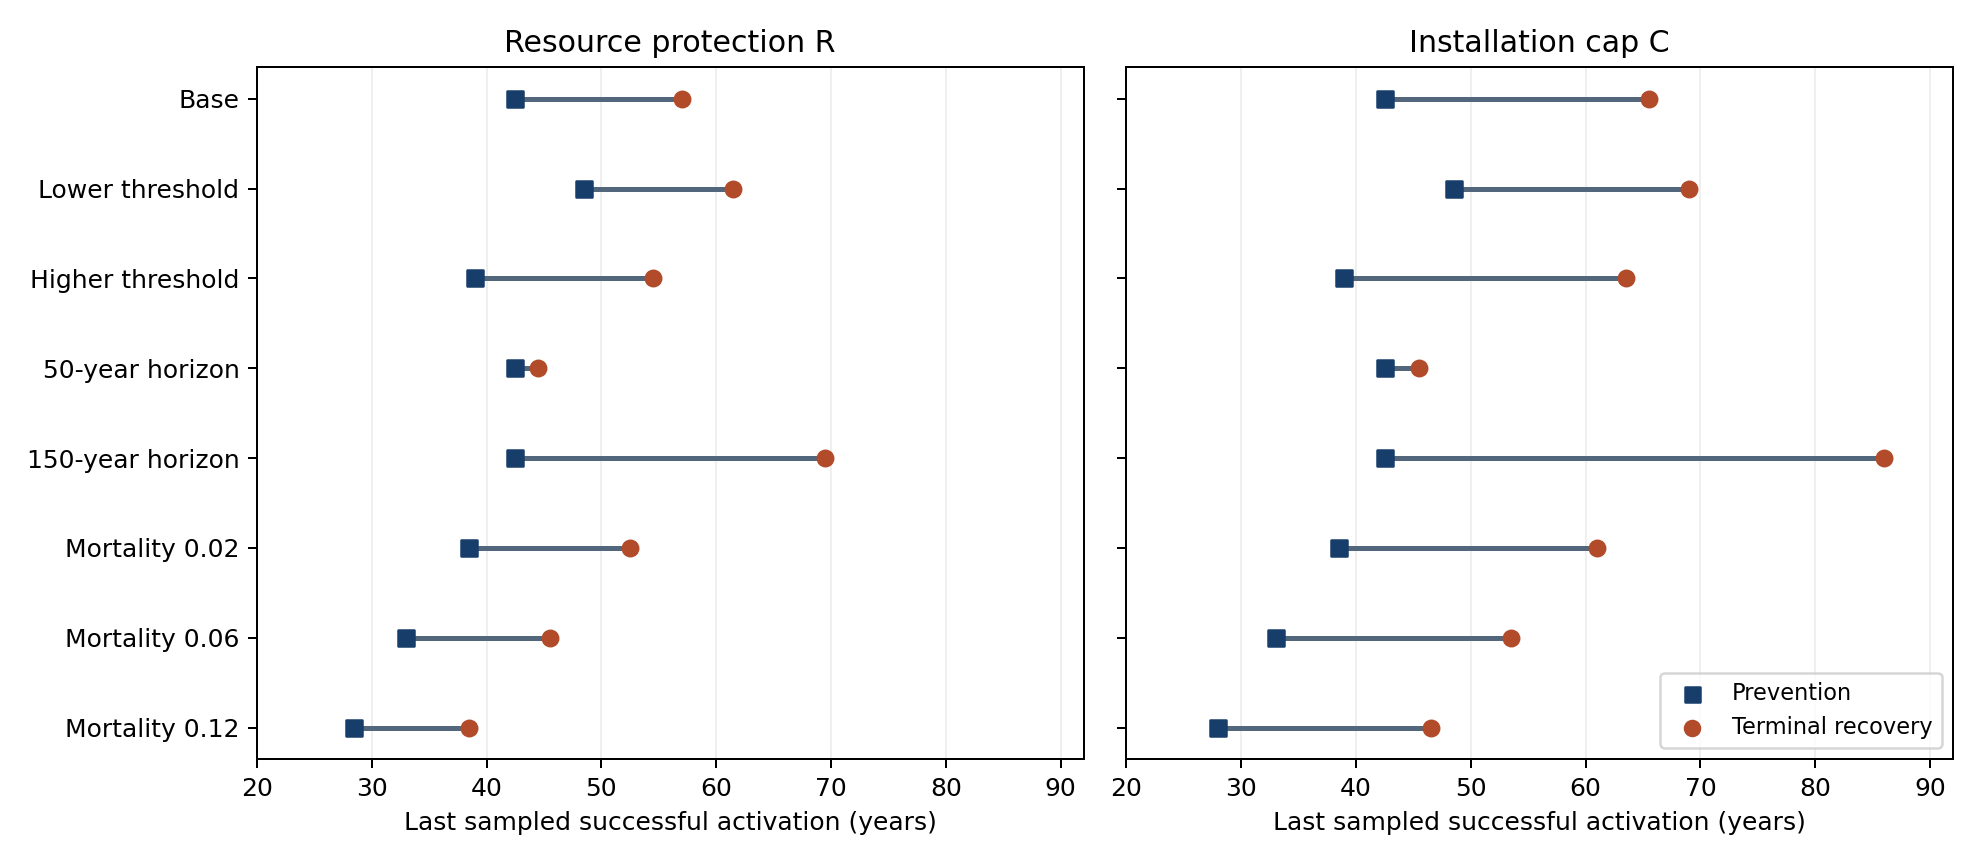
\includegraphics[width=0.93\linewidth]{review_sensitivity_windows.png}
\caption{Last successful sampled prevention and recovery starts under changes to the threshold, horizon, and shortage mortality. Segments show the gap between the two objectives; endpoints have 0.5-year sampling resolution.}\label{fig:sensitivity}
\end{figure}

\subsection{Outcome Classification and Model Structure}
We next test whether the finding that population protection can coexist with resource inadequacy depends on the evaluation standard. Lowering the adequacy threshold from 0.8 to 0.6 reclassifies some early-intervention trajectories from marginal to non-marginal survival without changing their population or resource trajectories. Outcome labels should therefore be reported alongside actual satisfaction levels.

In a separate check using eight AI parameter combinations, four untreated cases cross the population threshold. Early R or C prevents crossing in every case, but all remain classified as marginal survival. When either policy starts at year 50, four cases cross and later recover. These cases support the distinction between population protection, population recovery, and resource adequacy.

We also compare alternative allocation rules and capability growth with and without a fixed ceiling. Within the tested parameter sets, sufficiently strong protection keeps every case above the population safety floor, but no tested alignment level makes every case non-marginal. The protection required for population safety also changes with the parameter range. Thus, the distinction between safety and adequacy persists in these tests, while the specific safety level depends on the model setting.

\subsection{Numerical Accuracy}\label{sec:verification}
To check whether numerical error affects the intervention boundaries, we tighten solver tolerances and reduce time steps for eight cases near the prevention and recovery boundaries of R and C. Every success or failure classification remains unchanged. The maximum relative difference in terminal population is approximately $1.18\times10^{-5}$.

First threshold crossings are located through solver events, avoiding missed crossings between output times. Intervention starts are still scanned on a finite grid, however, so the reported boundaries reflect the sampling resolution rather than exact continuous critical times.


\section{Conclusions and Model Evaluation}

\subsection{Conclusion}

\textbf{Population protection does not guarantee resource adequacy.} Early resource protection and installation limits prevent threshold crossings in the tested pressure scenario, but population growth spreads fixed energy and land supplies across more people. Successful protection can therefore leave marginal survival. Policy evaluation must track resources per person alongside population.

\textbf{Prevention and terminal recovery have different deadlines.} In the 100-year pressure scenario, the latest successful sampled recovery starts are 14.5 years later than preventive starts for R and 23.25 years later for C. Hardware retirement releases energy, supporting faster late recovery under C in these cases; neither policy is universally preferable. Recovery does not erase earlier losses.

\textbf{The timing gap depends on the horizon and demographic response.} Longer horizons allow more recovery time, while deprivation mortality brings intervention deadlines forward. These are conditional opportunities, not universal dates. ENOCH should protect essential resources early and assess population losses, terminal recovery and resource adequacy separately.

\subsection{Model Evaluation and Limitations}

\textbf{Model strengths.} Resource allocation is coupled to population, hardware, and capability dynamics, allowing us to trace how competition affects long-term outcomes. Energy and land have separate constraints, and construction and operating electricity are accounted for separately, giving each intervention a clear physical interpretation. Population comparison bounds, a sufficient protection condition, and a necessary recovery bound also distinguish results established by the equations from those requiring scenario-specific simulation.

\textbf{Recovery depends on continued supply and enforcement.} The model assumes that electricity remains available and policies can be enforced after activation. Crossing the effective-extinction threshold does not automatically trigger irreversible infrastructure or institutional collapse. Severe decline could undermine these recovery conditions in practice, so the modeled recovery opportunities may be optimistic.

\textbf{Population and welfare remain simplified.} The model considers reduced recruitment and additional mortality under resource shortages, but does not explicitly represent age structure, lasting health damage, or delayed fertility responses. Resource satisfaction measures the provision of basic needs rather than overall quality of life or social recovery. Policy restrictions are also recorded in different physical units, including energy and hardware, which do not establish an economically optimal policy.

\textbf{Parameters and numerical results are conditional.} The historical model reproduces a compatible timescale, but coexistence time alone cannot identify the competition mechanism. RSI parameters are primarily scenario assumptions, and finite parameter sets and activation-time grids cannot cover all possibilities. Numerical accuracy checks support the stability of the tested cases, but sample frequencies are not real-world probabilities, and sampled deadlines are neither exact nor universal policy boundaries.

\subsection{Future Work}

We retain three priorities for extending the framework.

\textbf{Technological evolution.} Future models could allow changes in computing architecture to alter energy, hardware and land requirements per task. These gains should be considered alongside demand rebound: lower computing costs may encourage expansion and offset efficiency savings. This would test whether technological progress eases competition or mainly supports a larger AI sector.

\textbf{Demographic and social responses.} Age structure, lasting health damage and delayed fertility responses could improve estimates of decline and recovery after prolonged deprivation. Resource shortages, employment changes and inadequate public services may also generate pressure for intervention. Allowing policies to emerge from these pressures would support comparisons between proactive prevention and reactive intervention, rather than prescribing activation times externally.

\textbf{Institutional and policy dynamics.} Implementation delays and time-varying enforcement could represent differences in regulatory capacity, ownership, governance and international coordination. Severe decline may also damage electricity supply, facility maintenance and the institutions needed to act. Modeling these feedbacks, including irreversible losses, would test whether recovery remains feasible when resource provision and policy implementation depend on the evolving system.

\FloatBarrier
\clearpage
\section*{Letter to ENOCH}
\addcontentsline{toc}{section}{Letter to ENOCH}
\noindent Dear Members of the ENOCH Board,

Our model asks what would happen if recursively self-improving AI systems shared limited energy and land with humans. It does not predict whether such systems will exist. We find that human population, access to essential resources and the timing of intervention must be considered together.

Two actions were examined in detail: protecting a minimum human share of usable resources and limiting new AI hardware installation. In the pressure scenario, both can prevent a population-floor crossing when started early. However, the last start that prevents every crossing is earlier than the last start that permits population recovery by the end of the study. For the stated 100-year background, the tested gaps are about 14.5 years for resource protection and 23.25 years for the installation cap. These are conditional sampled results, not real-world deadlines.

A larger recovered population is not necessarily better provided for. With fixed supplies, early successful protection can increase population until resources per person again become inadequate. A late policy can also restore population above the effective-extinction floor after a previous crossing. Neither case proves that social institutions, public health or welfare have recovered. Avoiding the initial loss remains a distinct objective.

We have greater confidence in the conditional mathematical bounds than in any numerical year. The resource-protection certificate states assumptions under which a population floor cannot be crossed. Conversely, our recovery envelope identifies starts that are too late even under immediate full resource satisfaction. The numerical windows survived the tested alternatives, but changing the horizon from 50 to 150 years greatly expanded them, and adding deprivation-related mortality moved preventive deadlines earlier. Continued electricity supply and enforceable policies remain strong assumptions.

If one uncertain response could be measured first, we would prioritize the effect of sustained essential-service shortfall on human net population growth, especially additional mortality. This recommendation follows the sensitivity of the tested deadlines; it is not a formal value-of-information optimum. Better measurement would help distinguish genuine intervention time from time supplied by an optimistic demographic assumption.

A present-day use is assessing data-centre expansion against community electricity and land needs. The common allocation mechanism can identify which services bind and how construction competes with operation, after calibration with local data. Our advice is to protect essential access, preserve the ability to act before large losses occur, and monitor adequacy rather than interpreting population persistence alone as success.

\medskip
Sincerely,\\
Team \TeamNumber

\clearpage
\begin{thebibliography}{99}
\setlength{\itemsep}{0pt}
\setlength{\parsep}{0pt}
\setlength{\parskip}{0pt}
\addcontentsline{toc}{section}{References}
\bibitem{problem} EuroMCM. \emph{2026 Problem $\alpha$: Our Turn}. Competition problem statement supplied with the task, 2026.
\bibitem{kelly} F. P. Kelly. Charging and rate control for elastic traffic. \emph{European Transactions on Telecommunications}, 8:33--37, 1997. Corrected \href{https://www.statslab.cam.ac.uk/~fpk1/elastic.html}{Author version}.
\bibitem{aubin} J.-P. Aubin, A. M. Bayen and P. Saint-Pierre. \emph{Viability Theory: New Directions}, 2nd ed. Springer, 2011. \href{https://doi.org/10.1007/978-3-642-16684-6}{doi:\nolinkurl{10.1007/978-3-642-16684-6}}.
\bibitem{aghion} P. Aghion, B. F. Jones and C. I. Jones. \emph{Artificial Intelligence and Economic Growth}. NBER Working Paper 23928, 2017. \href{https://doi.org/10.3386/w23928}{doi:\nolinkurl{10.3386/w23928}}.
\bibitem{chen} Z. Chen, Y. Yang, J. Zhou, Q. Zhang, C.-T. Lin and Y. Duan. \emph{Survival Games: Human-LLM Strategic Showdowns under Severe Resource Scarcity}. arXiv:2505.17937, 2025. \href{https://arxiv.org/abs/2505.17937}{Preprint}.
\bibitem{higham} T. Higham et al. The timing and spatiotemporal patterning of Neanderthal disappearance. \emph{Nature}, 512:306--309, 2014. \href{https://doi.org/10.1038/nature13621}{doi:\nolinkurl{10.1038/nature13621}}.
\bibitem{djakovic} I. Djakovic, A. Key and M. Soressi. Optimal linear estimation models predict 1400--2900 years of overlap between Homo sapiens and Neandertals prior to their disappearance from France and northern Spain. \emph{Scientific Reports}, 2022. \href{https://doi.org/10.1038/s41598-022-19162-z}{doi:\nolinkurl{10.1038/s41598-022-19162-z}}.
\bibitem{iea} International Energy Agency. \emph{Energy and AI}. Paris, 2025. \href{https://www.iea.org/reports/energy-and-ai/energy-demand-from-ai}{Report}.
\bibitem{mellars} P. Mellars and J. C. French. Tenfold population increase in Western Europe at the Neandertal-to-modern human transition. \emph{Science}, 333(6042):623--627, 2011. \href{https://doi.org/10.1126/science.1206930}{doi:\nolinkurl{10.1126/science.1206930}}.
\bibitem{snodgrass} J. J. Snodgrass and W. R. Leonard. Neandertal energetics revisited: Insights into population dynamics and life history evolution. \emph{PaleoAnthropology}, 2009:220--237, 2009. \href{https://doi.org/10.4207/PA.2009.ART31}{doi:\nolinkurl{10.4207/PA.2009.ART31}}.
\bibitem{froehle} A. W. Froehle and S. E. Churchill. Energetic competition between Neandertals and anatomically modern humans. \emph{PaleoAnthropology}, 2009:96--116, 2009. \href{https://paleoanthro.org/media/journal/content/PA20090096.pdf}{Full text}.
\end{thebibliography}

\appendix
\noindent\begin{minipage}{\linewidth}
\section{Disclosed parameter ranges for scenario draws}\label{app:ranges}
U and L denote uniform and log-uniform sampling. The first three columns use 32 draws per range (seed 20261017); the last uses eight pressure-scenario draws (seed 2027). Only the eight listed RSI parameters vary. These exploratory distributions are not empirical estimates and are separate from the fixed-setting timing scans in Section~\ref{sec:sensitivity}.

\begingroup
\centering\footnotesize
\captionof{table}{Exploratory supports for the eight varying RSI parameters. Units are those of the model definitions.}\label{tab:ranges}
\begin{tabular}{@{}lllll@{}}\toprule
Parameter & Conservative & Central & Aggressive & Later stress\\\midrule
$\eta$ & $0.02$--$0.1$ (L) & $0.05$--$0.3$ (L) & $0.1$--$1$ (L) & $0.3$--$1$ (L)\\
$\xi$ & $0$--$0.3$ (U) & $0$--$0.5$ (U) & $0$--$0.5$ (U) & $0$--$0.1$ (U)\\
$\omega$ & $0$--$0.3$ (U) & $0$--$0.8$ (U) & $0.3$--$1.5$ (U) & $0.8$--$1.2$ (U)\\
$q_c$ & $8$--$20$ (L) & $5$--$15$ (L) & $3$--$10$ (L) & $3$--$8$ (L)\\
$M_{\max}$ & $1\!\times\!10^{4}$--$1\!\times\!10^{5}$ (L) & $1\!\times\!10^{4}$--$5\!\times\!10^{5}$ (L) & $1\!\times\!10^{5}$--$1\!\times\!10^{6}$ (L) & $5\!\times\!10^{5}$--$1\!\times\!10^{6}$ (L)\\
$c_A$ & $0.1$--$0.5$ (L) & $0.1$--$0.8$ (L) & $0.3$--$1$ (L) & $0.7$--$1$ (L)\\
$w_{A0}$ & $1$--$10$ (L) & $1$--$100$ (L) & $10$--$1\!\times\!10^{4}$ (L) & $3\!\times\!10^{3}$--$1\!\times\!10^{4}$ (L)\\
$e_0$ & $1\!\times\!10^{3}$--$5\!\times\!10^{3}$ (L) & $2\!\times\!10^{3}$--$1\!\times\!10^{4}$ (L) & $5\!\times\!10^{3}$--$2\!\times\!10^{4}$ (L) & $8\!\times\!10^{3}$--$2\!\times\!10^{4}$ (L)\\
\bottomrule\end{tabular}

\par
\endgroup
\end{minipage}

\clearpage
\section*{Report on Use of AI Tools}
\addcontentsline{toc}{section}{Report on Use of AI Tools}
% The competition statement excludes this report from the 25-page limit.
% Consolidate all team members' actual tool use before submission.
\textbf{Scope.} This report records AI assistance visible in the present modeling audit and manuscript-drafting work. The team must consolidate any additional tools used by other members before submitting a final disclosure. No team identities are included in this report.

\textbf{Tool.} OpenAI Codex assistant. The exact deployed model identifier is not independently recorded in this manuscript package and should be taken from the team's account or session record if required.

\textbf{Uses.} The assistant inspected local model code and saved numerical results; proposed and implemented event-based risk-adjudication changes; added a separately labeled deprivation-mortality alternative; generated sensitivity and boundary-check scripts; ran numerical experiments and regression tests; organized mathematical assumptions, propositions and proofs; drafted and revised English exposition, the summary and ENOCH letter; checked selected references using author, publisher, institutional and original-preprint pages; and assembled LaTeX source and figure dependencies.

\textbf{Representative requests.} The work included requests to assess model reasonableness and priorities; complete continuous-event corrections, sensitivity checks and mechanism explanations; identify mathematical contributions and a paper structure; and write local LaTeX source for later upload to Overleaf. The team supplied the EuroMCM reference LaTeX summary template during drafting.

\textbf{Numerical record.} The audit reported 84 passing tests, 621 additional timing-scan solves, eight boundary cases each evaluated at default and tighter settings, 25 trajectories supporting 175 risk-convention assessments, and a rerun of the 50 revised policy-grid cases. Counts describe implemented checks; they are not independent empirical observations or a global proof. Earlier stored results are distinguished from the current checks in the manuscript.

\textbf{Verification and responsibility.} AI-generated equations and prose require team review. Analytic results are accompanied by assumptions and proofs; numerical claims are tied to local outputs. Historical compatibility is not presented as causal validation, and conditional scenario frequencies are not real-world risk probabilities. The submitted document, references, competition compliance and all conclusions remain the team's responsibility.

\textbf{Source preparation.} The assistant assembled local LaTeX and checked source-level references and file dependencies. The manuscript was not compiled or visually validated in this drafting session, at the team's request to handle Overleaf compilation separately.
\end{document}
